\documentclass[11pt]{article}

\usepackage[utf8]{inputenc}
\usepackage[T1]{fontenc}
\usepackage[a4paper,margin=1in]{geometry}
\usepackage{amsmath,amssymb}
\usepackage{booktabs}
\usepackage{graphicx}
\usepackage{array}
\usepackage[hidelinks]{hyperref}
\usepackage[round]{natbib}

% Shrink-to-fit wrapper (base packages only): scales a box down to \linewidth
% only when it is too wide, otherwise leaves it at natural size.
\newsavebox{\fitbox}
\newcommand{\fitwidth}[1]{%
  \sbox{\fitbox}{#1}%
  \ifdim\wd\fitbox>\linewidth\resizebox{\linewidth}{!}{\usebox{\fitbox}}\else\usebox{\fitbox}\fi}

% Tables in this document keep the author's original (non-sequential) numbering,
% so captions are typeset manually rather than via \caption auto-numbering.
\newcommand{\tabcap}[2]{\noindent\textbf{#1} #2\par\smallskip}

\title{Unsupervised Anomaly Detection Methods for Syndromic Surveillance:\\
A Comparative Study on Simulated Data}
\author{}
\date{}

\begin{document}
\maketitle

\section{Introduction}

The early detection of public health incidents, including outbreaks, is a central objective of syndromic surveillance systems. The aberration detection algorithms currently deployed in national systems include the Farrington Flexible \citep{noufaily2013} and RAMMIE (rising activity, multilevel mixed effects, indicator emphasis) used by the UK Health Security Agency, and the Early Aberration Reporting System (EARS) used by the US CDC \citep{hutwagner2003, noufaily2013, morbey2015}. \citet{noufaily2019} compared these three methods against each other on simulated daily syndromic data. They concluded that, among variants maintaining high specificity, Farrington Flexible achieves the highest mean sensitivity and specificity while RAMMIE achieves the highest mean probability of detecting the outbreaks. However, these statistical methods are slow at detecting anomalies of smaller magnitudes and often fail to detect anomalies with small signal-to-noise ratios. By learning the distribution of normal surveillance counts without explicit parametric assumptions, machine learning models may detect these kind of anomalies.

This study extends the comparison of \citet{noufaily2019} by introducing unsupervised machine learning models as anomaly detectors, evaluated on the simulated data used by \citet{noufaily2019}. We benchmark against Farrington Flexible specifically because it was the strongest high-specificity method in that comparison. We also include other GLM-based methods, but RAMMIE and EARS, the other two methods in the \citet{noufaily2019} comparison, are not re-implemented here.

This chapter presents a systematic comparison of unsupervised anomaly detection methods applied to simulated daily syndromic surveillance count data. We evaluate 11 individual methods, including the Farrington Flexible reference method, that can be categorized into three families: density-based methods on tabular features, reconstruction-based deep learning models, and seasonal-baseline statistical detectors. We then evaluate OR-vote ensemble combinations of these methods. All methods are evaluated under identical data splits, operating-point calibration, and the evaluation metrics of \citet{noufaily2019}. The robustness of each method is assessed across three outbreak magnitude levels (small, medium, and large), providing evidence on which method families are most suitable for deployment across a range of outbreak scenarios.

The structure of this chapter is as follows. Section 2 describes the simulated dataset and the evaluation framework, including the metric definitions and threshold-tuning procedure. Section 3 presents each method family and the algorithms within it, including a residual-feature variant of the tabular detectors. Section 4 reports individual detector results, robustness across magnitudes, per-signal variation, ensemble configurations, and the residual-feature ablation. Section 5 discusses the implications of these results, including the mechanistic signal properties that govern method success and the limits of detectability. Section 6 concludes with recommendations for deployment.


\section{Experimental Setup}

\subsection{Data}

The evaluation uses a simulated daily-count syndromic surveillance dataset generated with the simulation framework of \citet{noufaily2019}, which builds on the data-generating model of \citet{noufaily2013}. This is the same framework used to compare the deployed statistical methods, ensuring that the machine learning detectors evaluated here are tested on identical data structures. The dataset comprises 16 syndromic indicators (hereafter \textit{signals}), each consisting of 500 independent simulation runs of 2,548 days (seven years of 364-day years). The 16 signals span the four service types reporting to Public Health England --- GP out-of-hours, GP in-hours, NHS 111, and emergency department --- and were parameterised (following Table 1 of \citealp{noufaily2019}) to cover the range of volume, trend, seasonality, and day-of-week structure seen across more than 12,000 real syndromic series. (The reference comparison used 100 simulations per signal; this study uses 500, increasing the precision of the per-signal estimates.)

\paragraph{Baseline process.} Each signal's non-outbreak counts are drawn from a Negative Binomial distribution with mean $\mu_t = \exp\{\theta + \beta t + s(t)\}$, where $\theta$ sets the baseline level, $\beta$ an optional linear trend, and $s(t)$ a sum of Fourier harmonics ($k_1$ annual and $k_2$ within-week terms) capturing annual seasonality and a within-week cycle. The dispersion parameter $\phi$ ranges from 1 (Poisson) to 4 across signals. The per-signal parameters reproduce the diversity of real surveillance streams: baseline levels span three orders of magnitude (from $\approx 1$ case/day for rubella to $\approx 600$ for urinary tract infection), seasonal amplitudes range from negligible (cardiac, hepatitis) to dominant (arthropod bites, allergic rhinitis), and overdispersion ranges from Poisson-like to highly overdispersed. Eight signals represent five-day (weekday) reporting services --- with weekends set to structural zeros and twin Monday/Friday peaks --- while the other eight represent seven-day services in which weekend volume is roughly a third to a half of weekday volume. Bank-holiday effects are applied to mimic real reporting artefacts.

\paragraph{Outbreak injection.} Outbreaks are added as clusters of cases whose temporal profile follows a log-normal(0, 0.5) shape binned to daily resolution, and whose total size is Poisson-distributed with mean $m$ times the standard deviation of the baseline count on the outbreak's start day (i.e.\ $m\sqrt{\phi\mu_t}$). Day-of-week weighting is applied to the injected cases, mirroring the baseline reporting pattern (e.g.\ a Monday excess for weekday services, a weekend doubling for seven-day services). The framework distinguishes \textit{spiked} outbreaks (lasting approximately three weeks on average) from longer \textit{seasonal} outbreaks (approximately eight weeks); for evaluation, a single spiked outbreak is injected at a random position within the final 49 weeks of each simulation, which is the period on which detection is scored. Three signals (allergic rhinitis, heat stroke, influenza-like illness) additionally carry recurring annual \textit{seasonal} outbreaks in the baseline period, making their non-outbreak dynamics deliberately harder to model.

\paragraph{Outbreak magnitude.} Three versions of the dataset were generated, labelled \textit{small}, \textit{medium}, and \textit{large}, corresponding to three increasing values of the size multiplier $m$, which scales the injected outbreak relative to the local baseline standard deviation. The small-magnitude setting represents the most operationally challenging scenario, in which outbreak signals are close to the natural variation of the baseline; the large setting produces outbreaks several baseline standard deviations in size. Because the injected size is scaled by $\sqrt{\phi\mu_t}$ and the cases may fall on low-reporting days (weekends, seasonal troughs) and are spread over several weeks by the log-normal profile, a fraction of small-magnitude outbreaks manifest as short, low-count label runs that are not separable from baseline variation even in principle; this is examined in Section 5.7.

Ground-truth outbreak labels are available for evaluation but are not used during model training (see Section 2.5).

\subsection{Data split}

An identical 60/20/20 split of simulations is applied across all methods and all signals using a shared pseudorandom number generator (\texttt{numpy.random.RandomState} with seed 42) and the \texttt{split\_60\_20\_20} utility function. This produces 300 training simulations, 100 validation simulations, and 100 test simulations per signal. The split is performed at the simulation level, not at the day level, so that entire time series are held out. This design prevents temporal information leakage between partitions.

\subsection{Evaluation window and metrics}

Test-set alarms are evaluated on the absolute day range [2205, 2548), corresponding to the final 49 weeks of each test simulation. This evaluation window, denoted \texttt{IDX\_RANGE}, matches the window used in the original Farrington and Noufaily evaluation studies.

Six metrics are computed, each averaged across all test simulations and all 16 signals:

\begin{enumerate}
\item \textbf{Sensitivity.} The proportion of injected outbreak days that are detected ($TP / P$, where $P$ is the total number of outbreak days). For consistency with \citet{noufaily2019} the denominator is computed over the full series, but because every injected outbreak lies within the evaluation window \texttt{IDX\_RANGE}, this is numerically identical to a window-restricted count (no outbreak days occur in the earlier years). Sensitivity is therefore evaluated over the same final-49-week window as specificity, and the reported values are straightforward per-window detection rates.

\item \textbf{Specificity.} The proportion of non-outbreak days within \texttt{IDX\_RANGE} on which no alarm is raised:
\[
\text{Specificity} = \frac{TN}{TN + FP}, \quad \text{restricted to } t \in \texttt{IDX\_RANGE}.
\]

\item \textbf{False positive rate (FPR).} The complement of specificity within \texttt{IDX\_RANGE}:
\[
\text{FPR} = \frac{FP}{FP + TN} = 1 - \text{Specificity}.
\]

\item \textbf{Probability of detection (POD).} The fraction of test simulations in which at least one true positive alarm is raised during the outbreak period. POD measures per-outbreak detection capability, as opposed to sensitivity which measures per-day detection.

\item \textbf{Timeliness.} For each simulation containing an outbreak, the delay between the first alarm and the outbreak start, normalised by the outbreak window length:
\[
\text{Timeliness} = \frac{t_{\text{first alarm}} - t_{\text{outbreak start}}}{t_{\text{outbreak end}} - t_{\text{outbreak start}}},
\]
averaged across simulations. A value of 0 indicates perfect timeliness (alarm on the first outbreak day); a value of 1 indicates that no alarm was raised during the outbreak window. Lower values are better. Note that this metric conflates two effects: the lateness of detection when an outbreak \textit{is} caught, and a miss penalty (a missed outbreak contributes the maximum value of 1). Because missed outbreaks dominate the average for low-sensitivity detectors, timeliness partly tracks the probability of detection; it should be read alongside POD rather than in isolation.

\item \textbf{Timely detection --- Probability of Successful Detection within $d$ days, PSD($d$).} Each simulation contains exactly one injected outbreak, placed inside the evaluation window, so the outbreak window of a simulation is the interval $[t_{\text{onset}}, t_{\text{end}}]$ between its first and last injected day. Writing the detection delay as $\delta = t_{\text{first alarm on an outbreak day}} - t_{\text{onset}}$ (in days; $\delta \geq 0$, with a miss when no alarm coincides with an outbreak day), the timely-detection metric is
\[
\mathrm{PSD}(d) = \Pr(\delta \leq d),
\]
the probability that the outbreak is detected no later than $d$ days after its onset. As $d \to \infty$, $\mathrm{PSD}(d) \to \mathrm{POD}$, so PSD decomposes the detection problem cleanly: the asymptote is the overall catch rate (POD) and the early slope is the speed. We also report the Conditional Expected Delay, $\mathrm{CED} = \mathbb{E}[\delta \mid \text{detected}]$, the mean delay over caught outbreaks. This family of measures is due to \citet{frisen2003} and reviewed by \citet{sonesson2003}. PSD is reported alongside specificity, because --- like sensitivity or POD --- it can be driven arbitrarily high by an indiscriminate detector and is only meaningful at a controlled false-alarm rate. Because each simulation carries a single outbreak, POD, timeliness, and PSD are all evaluated once per simulation; an earlier event-level analysis that split each outbreak into maximal runs of injected days was found to fragment one $\approx$2-week outbreak into a body plus isolated single-day ``satellite'' events, and is not used here (Section 5.7).
\end{enumerate}

\subsection{Operating-point calibration}

For every non-Farrington method, the validation partition is used to select an operating point by maximising the objective
\[
\mathcal{L}(\tau) = 2 \cdot \text{Sensitivity}(\tau) + 3 \cdot \text{Specificity}(\tau), \quad \text{subject to } \text{Specificity}(\tau) \geq 0.97,
\]
where $\tau$ denotes the candidate numeric score cutoff. For methods whose search grid is expressed as candidate contamination percentiles, each percentile is first converted to the corresponding validation-set score cutoff; the selected numeric cutoff is then applied unchanged to the held-out test scores. This represents the operational calibration step in which past confirmed outbreaks are used to set the sensitivity--specificity trade-off. The higher weight on specificity reflects the practical requirement that a surveillance system must maintain a low false-alarm rate to remain credible with epidemiologists. Hyperparameters and operating points are re-tuned independently for each outbreak magnitude. Farrington Flexible is not tuned by this criterion; it is run at its standard fixed operating point, $\alpha = 0.01$.

\subsection{Label usage and the definition of ``unsupervised''}

A method is classified as \textit{unsupervised at training time} if its model parameters are fitted without access to outbreak labels. Several methods in the seasonal-baseline family (CUSUM, BOCPD-residual, NB-HMM, Farrington) additionally exclude training-period outbreak days when fitting the seasonal baseline model. This constitutes a ``negative'' use of labels --- defining what is normal, rather than what is an outbreak --- and is standard practice in the surveillance literature. The threshold-tuning step (Section 2.4) uses outbreak labels on the validation set, but this is common to all methods and analogous to the operational calibration performed in deployed systems.

\subsection{Reproducibility}

All experiments use a fixed pseudorandom seed (\texttt{RNG\_STATE = 42}) for the simulation split, ensuring that every method is trained, calibrated, and evaluated on identical partitions. The metric implementation (reproducing that of \citealp{noufaily2019}), the 60/20/20 split utility, and all method runners are shared across detectors. Where ensemble configurations are selected, the selection is performed on the validation partition and reported on the held-out test partition (Section 4.5), so that no test-set information informs the choice of ensemble configuration. Deep learning models (LSTM-AE, VAE) are trained with seeded initialisation, though exact bit-level reproducibility is not guaranteed under GPU non-determinism. Software versions for the principal dependencies (scikit-learn, statsmodels, PyTorch, and the R \texttt{surveillance} package) are recorded with the released code.


\section{Methods}

The 11 individual methods evaluated in this study fall into three methodological families, described below.

\subsection{Density and distance-based methods on tabular features}

All methods in this family operate on a common 20-dimensional feature vector $\mathbf{x}_t \in \mathbb{R}^{20}$ constructed for each day $t$. The features comprise rolling means, medians, maxima, standard deviations, and median absolute deviations of the raw count series, computed over windows of 7, 14, and 21 days, together with day-over-day differences, lag-7 and lag-14 differences, and z-scores relative to a rolling baseline. These features encode the local statistical context of each day without requiring an explicit seasonal model.

\paragraph{Isolation Forest (IF).} The Isolation Forest algorithm \citep{liu2008} constructs an ensemble of random binary trees, each built by recursively selecting a random feature and a random split value. Anomalous observations, being few and distinct, are isolated in fewer splits and thus have shorter average path lengths. The anomaly score is a monotone decreasing transform of the mean path length across the ensemble, $s(x) = 2^{-\mathbb{E}[h(x)]/c(n)}$, where $h(x)$ is the isolation depth of $x$ and $c(n)$ is the expected path length in a tree built on $n$ points (used to normalise for sub-sample size); scores approaching 1 indicate anomalies and scores well below $0.5$ indicate inliers. Per-signal hyperparameter tuning is performed over a grid of window lengths, number of trees, maximum samples, and maximum features.

\paragraph{K-Nearest Neighbours (KNN).} The anomaly score for each observation is the Euclidean distance to its $k$-th nearest neighbour in the tabular feature space \citep{ramaswamy2000}. Observations that are far from their neighbours in the training distribution are flagged as anomalous. Per-signal tuning is performed over window length and $k$.

\paragraph{Local Outlier Factor (LOF).} LOF \citep{breunig2000} measures the local density of each observation relative to its neighbours. An observation whose local density is substantially lower than that of its neighbours receives a high LOF score. Unlike KNN, which uses absolute distance, LOF captures relative density, making it more robust to clusters of varying density. Per-signal tuning is performed over window length and $k$.

\paragraph{One-Class SVM (OCSVM).} The one-class support vector machine \citep{scholkopf2001} with a radial basis function (RBF) kernel learns the hyperplane that separates the training data from the origin in the kernel-induced feature space with maximum margin; the signed distance to this hyperplane serves as the anomaly score. The parameter $\nu \in (0,1]$ controls the trade-off, upper-bounding the fraction of training points allowed to fall on the anomalous side of the boundary (margin errors) and lower-bounding the fraction retained as support vectors. Per-signal tuning is performed over window length and $\nu$; the RBF kernel width uses scikit-learn's \texttt{gamma="scale"} convention throughout. For computational tractability, the OCSVM fit is capped at a random subsample of 30,000 training feature vectors when the full training matrix is larger.

\paragraph{Residual-feature variant.} A limitation of the tabular methods is that their features encode the seasonal cycle directly: on strongly seasonal signals, a winter peak produces feature values that resemble an outbreak, causing false alarms and masking genuine aberrations. As an ablation, the four tabular detectors (Isolation Forest, KNN, LOF, and One-Class SVM) were re-run on a residualised input stream. The raw count series is first passed through the same Negative Binomial seasonal-baseline GLM used by the statistical methods (Section 3.3), and the 20-dimensional feature vector is then constructed from the Pearson residuals $r_t$ rather than the raw counts $y_t$. This removes the annual cycle and day-of-week structure before feature construction, leaving outbreaks as the dominant departures from a near-stationary residual stream. The detector hyperparameter grids, feature definitions, validation calibration, and test evaluation are otherwise identical to the raw-count variants, isolating the effect of the input representation.

\subsection{Reconstruction-based deep learning methods}

Methods in this family train a neural network to reconstruct windows of the input time series. Observations that are poorly reconstructed --- yielding high reconstruction error --- are flagged as anomalous.

\paragraph{LSTM Autoencoder (LSTM-AE).} A bidirectional LSTM autoencoder with encoder dimensions 128, 64, and 32 and a latent dimension of 4, with a mirrored decoder. The model is trained using the Huber loss on non-outbreak training windows. The reconstruction error on each test day serves as the anomaly score. The model is implemented in PyTorch.

\paragraph{Variational Autoencoder with Negative Binomial output (VAE).} A one-dimensional convolutional encoder maps input windows to a latent Gaussian distribution; a convolutional decoder produces per-day parameters of a Negative Binomial distribution. The model is trained with an ELBO-style objective comprising the Negative Binomial reconstruction term and the Kullback--Leibler divergence between the approximate posterior and the prior. At scoring time, the most recent positions in the encoder input are masked so that the model predicts the current count from preceding context; the anomaly score is the averaged Negative Binomial negative log-likelihood over the masked tail of the window, rather than the full-window ELBO.

\paragraph{Per-signal model selection and training budget.} The released runners expose the principal capacity hyperparameters as configuration variables (VAE latent dimension; LSTM-AE latent dimension and width), allowing per-signal model searches to be run in the same validation-calibrated framework as the tabular methods. The reported deep-model tables use the cached selected configurations from that search, while the plain runners reproduce the default single-configuration setting. The search was intentionally small, with secondary hyperparameters (Kullback--Leibler weight, convolution width, window length) and the training budget held fixed for tractability; its marginal effect was small, at most about $+0.02$ sensitivity over a single fixed configuration. A separate budget check found that increasing the VAE training budget on a representative signal reduced reconstruction loss only marginally and did not materially change test sensitivity.

\subsection{Seasonal-baseline statistical methods}

The four residual-based methods in this family --- CUSUM, BOCPD-residual, NB-HMM, and RateChange-residual --- share a common first stage: a seasonal baseline is fitted to the training-period counts and each detector then operates on the residuals. For this baseline we use the standard harmonic (Serfling-type) seasonal regression that has long been the conventional baseline in surveillance \citep{serfling1963, unkel2012}: a Negative Binomial generalised linear model with a log link, annual and semi-annual Fourier harmonics, and day-of-week indicators, fitted on the outbreak-free training-period days. Its functional form --- log-linear seasonality with a within-week cycle --- is of the same broad class as the process that generated the data (Section 2.1); we therefore keep the baseline deliberately simple and pre-specified rather than tuning its complexity to the simulator, because a closer match to this particular generative process would inflate performance in a way that would not transfer to real surveillance data, where the true seasonal form is unknown. The fitted model provides a seasonal prediction $\hat{\mu}_t$ for each day $t$ together with an estimated dispersion $\hat{\phi}$ (the mean Pearson statistic of the training residuals), and the four methods differ only in how they post-process the standardised (Pearson) residuals
\[
r_t = \frac{y_t - \hat{\mu}_t}{\sqrt{\hat{\phi}\,\hat{\mu}_t}}.
\]
This baseline is a deliberately simple standard model rather than a tight fit, and in-sample diagnostics on the training residuals make its limits explicit: the overall level and the day-of-week cycle are well captured, but with two harmonics the model leaves residual annual autocorrelation on many signals (mean lag-364 autocorrelation $\approx 0.28$) and substantial within-week structure on the most strongly seasonal signals (lag-7 autocorrelation up to $0.77$ for influenza-like illness). This under-fitting is the direct mechanism behind the weaker performance of the residual-based detectors on those seasonal signals (Section 4.3), and it means they operate on imperfectly deseasonalised data rather than an idealised baseline.
Farrington Flexible is grouped with this family because it shares the same Negative Binomial seasonal-baseline philosophy, but it does \emph{not} use this baseline: it fits its own quasi-Poisson reference-window GLM internally (described below), whose seasonal structure is captured non-parametrically through multi-year reference windows rather than harmonic terms. Its baseline is therefore not aligned with the generative functional form, making it --- as the deployed reference --- the one detector in this family whose performance is not assisted by the baseline matching the simulator.

\paragraph{Farrington Flexible ($\alpha = 0.01$).} This is the \citet{noufaily2013} Farrington Flexible algorithm, the current reference method for aberration detection in national surveillance. The implementation used here inlines the custom Farrington routine so that it operates directly on the daily series while aggregating to weekly reference counts internally. It comprises the Farrington Flexible machinery used in the comparison: a quasi-Poisson GLM with a log link fitted to a ten-group seasonal reference window spanning the preceding $b = 5$ years with half-window $w = 3$ weeks; Anscombe-residual reweighting to downweight past aberrations during fitting; a linear time-trend term when enough non-zero historical data are available; a Negative Binomial predictive upper bound at significance level $\alpha = 0.01$ when overdispersion is present (Poisson otherwise); the exceedance statistic $X = (y_t - \hat{\mu}_t)/(U_t - \hat{\mu}_t)$ with an alarm raised when $X > 1$; and the \texttt{limit54} minimum-count filter that suppresses alarms when fewer than five cases are observed in the preceding four reference periods. Because it shares the same Negative Binomial seasonal-baseline philosophy as the other methods in this family, it is grouped here, but it is distinguished as the deployed-system reference against which the machine learning methods are benchmarked.

\paragraph{CUSUM (Negative Binomial seasonal).} A one-sided cumulative sum is computed on the Pearson residuals:
\[
S_t = \max(0, \; S_{t-1} + r_t - k),
\]
where $k$ is a per-signal slack parameter. An alarm is raised when $S_t$ exceeds a threshold. CUSUM accumulates evidence of sustained departures from the baseline, making it well-suited to gradual shifts but slow to respond to sudden spikes.

\paragraph{BOCPD-residual.} Bayesian Online Changepoint Detection, following the framework of \citet{adams2007}, is applied to the Pearson residuals under a Gaussian approximation with a Normal--Inverse-Gamma predictive model and a constant hazard rate selected on validation. The implemented anomaly score is the one-step-ahead predictive surprise, $-\log p(r_t \mid r_{1:t-1})$; larger values indicate that the current residual is unlikely under the posterior predictive distribution.

\paragraph{NB-HMM.} A two-state Hidden Markov Model in which state 0 (normal) emits a Negative Binomial distribution centred on the seasonal baseline mean $\hat{\mu}_t$, and state 1 (outbreak) emits the same distribution with mean inflated to $c \cdot \hat{\mu}_t$, where $c > 1$ is selected on validation. The emission dispersion is tied to the Pearson dispersion estimated from the baseline fit rather than learned from labels. The forward algorithm provides the posterior probability $P(\text{state}_t = 1 \mid y_{1:t})$, which serves as the anomaly score.

\paragraph{RateChange-residual.} The Pearson residuals $r_t$ are smoothed by a causal exponentially weighted moving average, $m_t = \alpha\,r_{t-1} + (1-\alpha)\,m_{t-1}$ (with $\alpha = 0.2$, fixed at a conventional EWMA value rather than tuned), and the anomaly score is the deviation of the current residual from this smoothed recent level, $z_t = r_t - m_t$, with an alarm raised on large positive excursions. Because $m_t$ depends only on past residuals, the score responds to the \textit{rate of change} at outbreak onset rather than the sustained level: it fires on the rising edge and then falls silent as the EWMA adapts, which gives it strong timeliness but low day-level sensitivity.

\subsection{Ensemble methods}

\paragraph{OR-vote ensembles.} Each constituent detector independently calibrates its own alarm threshold or operating point on the validation set (Section 2.4). The ensemble alarm for day $t$ is the logical OR of the individual detector alarms:
\[
A_t^{\text{ens}} = \max(A_t^{(1)}, A_t^{(2)}, \ldots, A_t^{(K)}),
\]
where $A_t^{(k)} \in \{0, 1\}$ is the alarm from detector $k$. This strategy maximises sensitivity at the cost of compounding false positives across detectors. The validation-selected search reported below enumerates two- to five-method subsets of the detectors with complete aligned validation and test outputs.

Exploratory score-level aggregation strategies --- mean-z normalisation (averaging robust z-scores across detectors) and max-z (taking the maximum z-score) --- were also tried during development, but the reproducible ensemble analysis reported here is restricted to OR-voting because it is simpler, directly auditable from binary alarm matrices, and consistently dominated the exploratory score-level variants.


\section{Results}

\subsection{Individual detector performance at medium outbreak magnitude}

Table 1 presents the performance of all 11 individual detectors and two OR-vote ensemble configurations at medium outbreak magnitude, sorted by sensitivity. All values are means across 16 signals.

\tabcap{Table 1.}{Performance of unsupervised anomaly detection methods at medium outbreak magnitude. Metrics are averaged across 16 signals. Methods are sorted by sensitivity in descending order.}

\begin{center}
\fitwidth{%
\begin{tabular}{clcccccl}
\toprule
Rank & Method & Sensitivity & Specificity & POD & Timeliness & FPR & Family \\
\midrule
1 & OR-vote (Farrington+IF+LSTM-AE+NB-HMM) & 0.857 & 0.940 & 0.992 & 0.094 & 0.060 & ensemble \\
2 & OR-vote (IF+LSTM-AE+NB-HMM) & 0.853 & 0.948 & 0.991 & 0.097 & 0.052 & ensemble \\
3 & KNN & 0.750 & 0.975 & 0.938 & 0.178 & 0.025 & tabular \\
4 & LSTM-AE & 0.711 & 0.976 & 0.879 & 0.240 & 0.024 & deep learning \\
5 & LOF & 0.703 & 0.974 & 0.913 & 0.211 & 0.026 & tabular \\
6 & Isolation Forest & 0.678 & 0.975 & 0.951 & 0.162 & 0.025 & tabular \\
7 & NB-HMM & 0.633 & 0.976 & 0.926 & 0.181 & 0.024 & statistical \\
8 & OCSVM & 0.617 & 0.974 & 0.913 & 0.214 & 0.026 & tabular \\
9 & Farrington ($\alpha=0.01$) & 0.556 & 0.979 & 0.931 & 0.215 & 0.021 & statistical \\
10 & VAE (NegBin) & 0.516 & 0.973 & 0.974 & 0.132 & 0.027 & deep learning \\
11 & CUSUM & 0.460 & 0.974 & 0.651 & 0.485 & 0.026 & statistical \\
12 & RateChange-residual & 0.272 & 0.977 & 0.984 & 0.088 & 0.023 & statistical \\
13 & BOCPD-residual & 0.212 & 0.973 & 0.962 & 0.112 & 0.027 & statistical \\
\bottomrule
\end{tabular}
}
\end{center}

Among individual detectors, KNN achieves the highest sensitivity (0.750), followed by LSTM-AE (0.711), LOF (0.703), and Isolation Forest (0.678). All individual detectors maintain specificity above 0.97, with false positive rates between 0.014 and 0.028. The Farrington method at $\alpha=0.01$ retains high specificity (0.979) but ranks ninth overall in sensitivity (0.556).

The OR-vote ensembles substantially outperform every individual detector. The four-detector ensemble (Farrington + IF + LSTM-AE + NB-HMM) achieves sensitivity 0.857 with timeliness 0.094, compared to the best individual detector's sensitivity of 0.750. This improvement comes at the cost of a higher false positive rate (0.060 vs.\ approximately 0.025 for individual detectors).

\subsection{Robustness across outbreak magnitudes}

To assess whether detection performance generalises across outbreak intensities, all methods were re-evaluated on medium and large outbreak magnitudes with independently re-tuned hyperparameters and alarm thresholds. Table 2 presents sensitivity and timeliness across the three magnitudes for all 11 individual detectors.

\tabcap{Table 2.}{Sensitivity and timeliness of individual detectors across three outbreak magnitudes. $\Delta$ Sens denotes the change in sensitivity from small to large magnitude. Methods are sorted by large-magnitude sensitivity.}

\begin{center}
\fitwidth{%
\begin{tabular}{lccccccc}
\toprule
Method & Sens (S) & Sens (M) & Sens (L) & Tim (S) & Tim (M) & Tim (L) & $\Delta$ Sens \\
\midrule
KNN & 0.615 & 0.750 & 0.854 & 0.281 & 0.178 & 0.099 & +0.239 \\
Isolation Forest & 0.523 & 0.678 & 0.827 & 0.291 & 0.162 & 0.085 & +0.304 \\
LSTM-AE & 0.570 & 0.711 & 0.816 & 0.374 & 0.240 & 0.133 & +0.245 \\
OCSVM & 0.464 & 0.617 & 0.787 & 0.355 & 0.214 & 0.090 & +0.323 \\
NB-HMM & 0.522 & 0.633 & 0.731 & 0.310 & 0.181 & 0.106 & +0.209 \\
LOF & 0.565 & 0.703 & --- & 0.326 & 0.211 & --- & +0.138* \\
Farrington ($\alpha=0.01$) & 0.440 & 0.556 & 0.639 & 0.378 & 0.215 & 0.128 & +0.199 \\
VAE (NegBin) & 0.424 & 0.516 & 0.611 & 0.226 & 0.132 & 0.080 & +0.187 \\
CUSUM & 0.404 & 0.460 & 0.393 & 0.533 & 0.485 & 0.571 & -0.011 \\
RateChange-residual & 0.234 & 0.272 & 0.294 & 0.153 & 0.088 & 0.047 & +0.060 \\
BOCPD-residual & 0.175 & 0.212 & 0.291 & 0.198 & 0.112 & 0.051 & +0.116 \\
\bottomrule
\end{tabular}
}
\end{center}

\noindent\textit{*LOF large-magnitude evaluation did not complete; the small-to-medium gain is reported.}

\medskip

Three distinct scaling tiers emerge from these results:

\begin{enumerate}
\item \textit{Strong scaling} ($\Delta\text{Sens} \geq +0.20$): the four tabular methods (IF +0.304, OCSVM +0.323, KNN +0.239) and LSTM-AE (+0.245). These methods gain 20--32 percentage points of sensitivity from small to large magnitude.

\item \textit{Moderate scaling} ($\Delta\text{Sens}$ between +0.15 and +0.20): NB-HMM (+0.209), Farrington (+0.199), and VAE (+0.187).

\item \textit{Weak or flat scaling}: BOCPD-residual (+0.116), RateChange (+0.060), and CUSUM ($-0.011$). The two pure onset detectors (CUSUM, RateChange) gain little from larger outbreaks because they respond to the rate of change at onset rather than the sustained level; BOCPD-residual scales modestly.
\end{enumerate}

At large magnitude, the top three individual detectors --- KNN (0.854), Isolation Forest (0.827), and LSTM-AE (0.816) --- all achieve sensitivity above 0.80, with timeliness below 0.14, while maintaining fully unsupervised training.

\subsection{Per-signal variation in detection performance}

The results presented in Sections 4.1 and 4.2 are averages across 16 signals. However, the 16 syndromic indicators represent diverse surveillance streams --- ranging from GP in-hours consultations (allergic rhinitis, herpes zoster) to NHS 111 calls (diarrhoea) and GP out-of-hours presentations (influenza-like illness, bronchitis) --- and detection performance varies substantially across them. This section examines per-signal variation, which is critical for understanding whether a method that performs well on average might fail on specific signals of operational importance.

Table 6 presents the per-signal sensitivity of nine key detectors at small outbreak magnitude.

\tabcap{Table 6.}{Per-signal sensitivity at small outbreak magnitude for nine detectors. Signals are grouped by difficulty: \textit{easy} (mean sensitivity across methods $> 0.70$), \textit{medium} (0.35--0.70), and \textit{hard} ($< 0.35$). The highest sensitivity per signal is shown in bold.}

\begin{center}
\fitwidth{%
\begin{tabular}{clcccccccccl}
\toprule
Sig & Indicator & Farr. & IF & KNN & OCSVM & LOF & LSTM & NB-HMM & VAE & CUSUM & Difficulty \\
\midrule
14 & Hepatitis, GPOOH & 0.904 & 0.908 & 0.902 & 0.897 & 0.842 & 0.882 & \textbf{0.940} & 0.873 & 0.210 & easy \\
7 & Herpes zoster, GP & 0.466 & 0.917 & \textbf{0.921} & 0.878 & 0.914 & 0.902 & 0.881 & 0.553 & 0.305 & easy \\
4 & ICU cardiac adm., ED & 0.760 & 0.769 & 0.738 & 0.760 & 0.660 & 0.691 & \textbf{0.844} & 0.673 & 0.776 & easy \\
12 & Upper resp.\ tract, GP & 0.585 & 0.853 & \textbf{0.873} & 0.829 & 0.846 & 0.849 & 0.835 & 0.440 & 0.415 & easy \\
3 & Cardiac, ED & 0.533 & 0.724 & \textbf{0.840} & 0.669 & 0.809 & 0.835 & 0.199 & 0.341 & 0.252 & medium \\
13 & Bronchitis, GPOOH & 0.694 & 0.358 & 0.572 & 0.520 & 0.725 & \textbf{0.800} & 0.536 & 0.735 & 0.000 & medium \\
16 & UTI, GPOOH & 0.535 & 0.556 & \textbf{0.681} & 0.535 & 0.594 & 0.486 & 0.422 & 0.359 & 0.502 & medium \\
9 & Pertussis, GP & 0.524 & 0.433 & 0.549 & 0.400 & 0.439 & 0.466 & 0.678 & 0.251 & \textbf{0.697} & medium \\
1 & Diarrhoea, NHS 111 & 0.375 & 0.475 & 0.618 & 0.237 & 0.639 & \textbf{0.666} & 0.302 & 0.313 & 0.338 & medium \\
2 & Arthropod bites, ED & 0.525 & 0.369 & 0.331 & 0.330 & 0.280 & 0.405 & 0.626 & 0.513 & \textbf{0.627} & medium \\
5 & Allergic rhinitis, GP & 0.119 & 0.634 & \textbf{0.860} & 0.289 & 0.723 & 0.594 & 0.247 & 0.406 & 0.012 & medium \\
11 & Rubella, GP & 0.500 & 0.367 & 0.347 & 0.331 & 0.095 & 0.214 & 0.616 & 0.366 & \textbf{0.694} & medium \\
10 & Pneumonia, GPOOH & 0.113 & 0.272 & \textbf{0.594} & 0.184 & 0.576 & 0.500 & 0.520 & 0.145 & 0.587 & medium \\
8 & Insect bite, GP & 0.075 & 0.253 & 0.432 & 0.180 & 0.337 & 0.274 & 0.417 & 0.221 & \textbf{0.689} & hard \\
6 & Heat stroke, GP & 0.174 & 0.260 & 0.270 & 0.213 & 0.169 & 0.216 & 0.172 & 0.182 & \textbf{0.355} & hard \\
15 & ILI, GPOOH & 0.157 & 0.217 & 0.309 & 0.179 & 0.385 & 0.346 & 0.112 & \textbf{0.417} & 0.010 & hard \\
\bottomrule
\end{tabular}
}
\end{center}

Several patterns emerge from Table 6. First, cross-signal variation is large for every method. The coefficient of variation (standard deviation divided by mean) of per-signal sensitivity ranges from 0.36 (KNN) to over 0.6 (CUSUM, Farrington Flexible), indicating that no method performs uniformly across signals. The sensitivity range (maximum minus minimum) exceeds 0.65 for every method.

Second, four signals are consistently easy to detect: hepatitis (signal 14), herpes zoster (signal 7), ICU cardiac admissions (signal 4), and upper respiratory tract infection (signal 12). These signals achieve mean sensitivity above 0.70 across all methods. Conversely, three signals are consistently hard: heat stroke (signal 6), insect bites (signal 8), and influenza-like illness (signal 15), with mean sensitivity below 0.35 at small magnitude. The easy signals likely have larger outbreak-to-baseline ratios or more distinctive outbreak temporal profiles; the hard signals may have high natural variability or small outbreak magnitudes relative to their baseline counts.

Third, the best-performing method varies across signals. The tabular methods (KNN, IF, LOF) dominate on the higher-volume signals with weak-to-moderate seasonality (herpes zoster, upper respiratory tract infection, cardiac, allergic rhinitis), where KNN alone is the best detector on six of the sixteen signals. The statistical methods occupy the complementary niche: NB-HMM is best on the high-SNR, low-overdispersion signals (hepatitis, ICU cardiac admissions), while CUSUM --- despite the lowest mean sensitivity of the tabular/statistical detectors --- is the single best detector on five signals (arthropod bites, heat stroke, insect bites, pertussis, rubella), all of them low-count and/or strongly seasonal, where its cumulative-sum mechanism captures gradual onset outbreaks. CUSUM nonetheless fails completely on bronchitis (0.000) and near-completely on allergic rhinitis (0.012) and ILI (0.010), so its strong per-signal wins coexist with catastrophic failures; this extreme signal-dependence means CUSUM is valuable within an ensemble but should not be deployed standalone. Notably, Farrington Flexible --- although competitive on several signals --- is not the single best detector on any signal at small magnitude, reflecting that its conservative, specificity-preserving operating point trades away sensitivity.

Fourth, the per-signal results explain why OR-vote ensembles outperform individual methods. No single method is best on more than six of the sixteen signals, and the wins are split across method families: KNN on signals 3, 5, 7, 10, 12, and 16; CUSUM on signals 2, 6, 8, 9, and 11; NB-HMM on signals 4 and 14; LSTM-AE on signals 1 and 13; and VAE on signal 15. The tabular and statistical families are therefore strongly complementary --- KNN covers the higher-volume, less-seasonal signals while CUSUM and NB-HMM cover the low-count and seasonal ones --- and the OR-vote ensemble captures the union of these per-signal strengths.

Table 7 shows how the per-signal sensitivity landscape changes at large outbreak magnitude.

\tabcap{Table 7.}{Per-signal sensitivity at large outbreak magnitude for seven detectors.}

\begin{center}
\fitwidth{%
\begin{tabular}{clccccccc}
\toprule
Sig & Indicator & IF & KNN & OCSVM & LSTM-AE & NB-HMM & VAE & CUSUM \\
\midrule
14 & Hepatitis, GPOOH & 0.918 & 0.921 & 0.917 & 0.924 & \textbf{0.932} & 0.906 & 0.118 \\
4 & ICU cardiac adm., ED & 0.925 & 0.914 & 0.922 & 0.917 & \textbf{0.956} & 0.786 & 0.482 \\
9 & Pertussis, GP & \textbf{0.931} & 0.922 & 0.923 & 0.917 & 0.919 & 0.435 & 0.694 \\
2 & Arthropod bites, ED & 0.748 & 0.754 & 0.716 & 0.754 & \textbf{0.895} & 0.819 & 0.253 \\
1 & Diarrhoea, NHS 111 & 0.833 & \textbf{0.891} & 0.703 & 0.842 & 0.652 & 0.603 & 0.602 \\
8 & Insect bite, GP & 0.732 & \textbf{0.884} & 0.595 & 0.721 & 0.812 & 0.472 & 0.640 \\
13 & Bronchitis, GPOOH & 0.794 & \textbf{0.894} & 0.868 & 0.848 & 0.583 & 0.776 & 0.000 \\
3 & Cardiac, ED & \textbf{0.873} & 0.872 & 0.855 & 0.863 & 0.749 & 0.640 & 0.751 \\
16 & UTI, GPOOH & \textbf{0.877} & 0.874 & 0.872 & 0.801 & 0.643 & 0.562 & 0.250 \\
12 & Upper resp.\ tract, GP & 0.864 & \textbf{0.865} & 0.855 & 0.820 & 0.805 & 0.546 & 0.154 \\
11 & Rubella, GP & 0.850 & 0.861 & \textbf{0.873} & 0.837 & 0.873 & 0.649 & 0.515 \\
7 & Herpes zoster, GP & 0.860 & \textbf{0.867} & 0.853 & 0.850 & 0.843 & 0.474 & 0.158 \\
5 & Allergic rhinitis, GP & 0.809 & \textbf{0.840} & 0.701 & 0.751 & 0.373 & 0.507 & 0.217 \\
10 & Pneumonia, GPOOH & 0.784 & \textbf{0.836} & 0.706 & 0.795 & 0.801 & 0.391 & 0.789 \\
6 & Heat stroke, GP & \textbf{0.766} & 0.723 & 0.648 & 0.627 & 0.587 & 0.468 & 0.409 \\
15 & ILI, GPOOH & 0.665 & 0.744 & 0.588 & \textbf{0.784} & 0.269 & 0.749 & 0.261 \\
\midrule
 & \textbf{Mean} & \textbf{0.827} & \textbf{0.854} & \textbf{0.787} & \textbf{0.816} & \textbf{0.731} & \textbf{0.611} & \textbf{0.393} \\
\bottomrule
\end{tabular}
}
\end{center}

At large magnitude, cross-signal variation is substantially reduced for the tabular and deep learning methods. The coefficient of variation for KNN drops from 0.36 at small magnitude to 0.06 at large magnitude; for Isolation Forest, from 0.46 to 0.09. This convergence indicates that the hard signals at small magnitude (heat stroke, insect bites, ILI) become detectable when outbreak signals are sufficiently large. The improvement is dramatic for some signals: Isolation Forest on heat stroke rises from 0.260 to 0.766 (+0.506); KNN on rubella rises from 0.347 to 0.861 (+0.514); LSTM-AE on rubella rises from 0.214 to 0.843 (+0.629).

However, CUSUM and NB-HMM retain high cross-signal variation even at large magnitude. CUSUM on bronchitis remains at 0.000, and NB-HMM on ILI remains at 0.269. The statistical methods' per-signal variation reflects the quality of the seasonal baseline fit: where the Negative Binomial GLM provides a good model of the non-outbreak dynamics, these methods perform well; where it does not (e.g., ILI with its irregular seasonal pattern), they underperform regardless of outbreak magnitude.

\subsection{Ensemble performance across magnitudes}

The detailed ensemble analysis below (Section 4.5) is conducted at small outbreak magnitude, where ensembles provide their greatest benefit. The two headline ensembles were also evaluated at medium and large magnitudes, using the magnitude-aligned per-detector alarms (Table 3). The ensemble's \textit{relative} advantage over individual detectors necessarily narrows as outbreak magnitude grows: individual tabular detectors scale strongly with magnitude (Table 2; e.g.\ Isolation Forest from 0.523 to 0.827, KNN from 0.615 to 0.854), whereas the ensembles are already strong at small magnitude and bounded above by the detectability ceiling (Section 5.7). Consequently, the gap between the best single detector and the best ensemble contracts from approximately 17 percentage points at small magnitude (0.78 vs.\ KNN 0.615) to about five points at large magnitude (0.90 vs.\ KNN 0.854).

\tabcap{Table 3.}{Cross-magnitude sensitivity, with small-magnitude timeliness and FPR, for the two headline OR-vote ensembles, computed from the magnitude-aligned per-detector alarms.}

\begin{center}
\fitwidth{%
\begin{tabular}{lccccc}
\toprule
Ensemble & Sens (S) & Sens (M) & Sens (L) & Tim (S) & FPR (S) \\
\midrule
OR-vote (Farrington+IF+LSTM-AE+NB-HMM) & 0.783 & 0.857 & 0.903 & 0.141 & 0.068 \\
OR-vote (IF+LSTM-AE+NB-HMM) & 0.770 & 0.853 & 0.902 & 0.146 & 0.060 \\
\bottomrule
\end{tabular}
}
\end{center}

\subsection{Combinatorial ensemble search with validation-based selection}

To identify the most effective OR-vote ensemble, all 2--5 element subsets of seven base detectors (Farrington Flexible, IF, LSTM-AE, NB-HMM, BOCPD-residual, CUSUM, VAE) were evaluated --- 112 configurations in total. Two methodological safeguards distinguish this analysis. First, to avoid selection-on-test bias, each configuration's metrics were computed on \textit{both} the validation and test partitions; the winning configuration at each operating point is chosen by its \textbf{validation} sensitivity and its \textbf{test} metrics are then reported. This ensures that no test-set information informs the choice of which detectors to combine. Second, every constituent detector's alarm threshold is tuned on validation alone (Section 2.4), and Farrington Flexible alarms are generated on the matching data magnitude --- correcting an earlier alignment error in which test-window alarms from the wrong magnitude inflated Farrington-containing ensembles by 8--17 percentage points.

Table 8 reports the validation-selected ensembles at three operating constraints, together with the lowest-cost configurations meeting the standard specificity floor. All sensitivities are test-set values.

\tabcap{Table 8.}{Validation-selected OR-vote ensembles at small outbreak magnitude. Each row is the configuration maximising \textit{validation} sensitivity subject to the stated constraint; \textit{test} metrics are reported. Cost tiers: \textit{cheap} ($< 30$ min, no GPU), \textit{medium} (1--2 h, no GPU), \textit{expensive} (requires GPU).}

\begin{center}
\fitwidth{%
\begin{tabular}{llccccl}
\toprule
Selection constraint & Ensemble (val-selected) & Sensitivity & Specificity & FPR & Timeliness & Cost \\
\midrule
Max sensitivity (spec $\geq 0.93$) & Farrington + IF + LSTM-AE + NB-HMM & 0.783 & 0.932 & 0.068 & 0.141 & expensive \\
Highest-sens Farrington-free (spec $\geq 0.93$) & IF + LSTM-AE + NB-HMM & 0.770 & 0.940 & 0.060 & 0.146 & expensive \\
Balanced (spec $\geq 0.95$) & LSTM-AE + NB-HMM & 0.735 & 0.954 & 0.046 & 0.190 & expensive \\
Best GPU-free (spec $\geq 0.95$) & IF + NB-HMM & 0.694 & 0.954 & 0.046 & 0.160 & medium \\
Best all-cheap (spec $\geq 0.96$) & Farrington + NB-HMM & 0.615 & 0.962 & 0.038 & 0.226 & cheap \\
\bottomrule
\end{tabular}
}
\end{center}

The best OR-vote ensembles reach test sensitivity 0.77--0.78 at the most permissive operating point (specificity $\approx 0.93$), comfortably exceeding the best single detector (KNN, 0.615). A paired cluster bootstrap over the 16 signals confirms that the ensemble advantage is statistically reliable: the recommended Farrington + IF + NB-HMM ensemble (test sensitivity 0.725) exceeds KNN by $+0.110$ (95\% CI $[+0.038, +0.186]$, $p < 0.01$). The advantage is, however, smaller than earlier (uncorrected) figures suggested, and it is purchased at a specificity cost: the high-sensitivity ensembles operate near specificity 0.93--0.95, against $\approx 0.97$ for the single detectors.

After alarm-magnitude alignment and validation-based selection, the strongest configuration at the high-sensitivity operating point is the four-detector Farrington + IF + LSTM-AE + NB-HMM (0.783), with the Farrington-free IF + LSTM-AE + NB-HMM close behind (0.770); the lower-cost Farrington + IF + NB-HMM (0.725) remains a competitive option. Farrington Flexible contributes genuine complementary coverage, because its NB-quantile exceedance rule fires on different events than the HMM posterior or the feature-space distance.

\subsection{Residual-feature variant on seasonal signals}

The per-signal analysis (Section 4.3) showed that the tabular methods systematically underperform on strongly seasonal signals. To test whether this weakness is attributable to the input representation rather than the detectors themselves, all four tabular detectors (Isolation Forest, KNN, LOF, and One-Class SVM) were re-run on Pearson residuals from the Negative Binomial seasonal baseline (Section 3.1, \textit{Residual-feature variant}). Table 10 reports the effect, stratified by signal type.

\tabcap{Table 10.}{Effect of residualising the input on tabular-method sensitivity, small outbreak magnitude. Signals are grouped into strongly seasonal (signals 2, 5, 6, 8, 13, 15; relative seasonal amplitude $\geq 0.5$) and the remaining low-seasonal signals.}

\begin{center}
\fitwidth{%
\begin{tabular}{llccc}
\toprule
Method & Signal group & Raw-count sens & Residual-feature sens & $\Delta$ \\
\midrule
Isolation Forest & Seasonal (6 signals) & 0.348 & 0.495 & \textbf{+0.146} \\
Isolation Forest & Low-seasonal (10 signals) & 0.627 & 0.627 & $-0.001$ \\
KNN & Seasonal (6 signals) & 0.462 & 0.625 & \textbf{+0.163} \\
KNN & Low-seasonal (10 signals) & 0.706 & 0.747 & +0.041 \\
LOF & Seasonal (6 signals) & 0.436 & 0.512 & \textbf{+0.075} \\
LOF & Low-seasonal (10 signals) & 0.641 & 0.689 & +0.048 \\
One-Class SVM & Seasonal (6 signals) & 0.285 & 0.511 & \textbf{+0.225} \\
One-Class SVM & Low-seasonal (10 signals) & 0.572 & 0.669 & +0.097 \\
\bottomrule
\end{tabular}
}
\end{center}

Residualisation improves every tabular detector on exactly the strongly seasonal signals where the raw-count features fail: Isolation Forest gains +0.146, KNN +0.163, LOF +0.075, and One-Class SVM +0.225. The gain is largest for One-Class SVM, which is the weakest raw-count detector on these signals (0.285), confirming that the limitation lies in the input representation rather than any single algorithm. On low-seasonal signals the effect ranges from negligible (Isolation Forest, $-0.001$) to modestly positive (KNN +0.041, LOF +0.048, One-Class SVM +0.097); for the two weaker detectors, LOF and One-Class SVM, residualisation therefore helps somewhat across the board rather than only on seasonal signals. The single largest improvement is Isolation Forest on bronchitis (signal 13), which rises from 0.358 to 0.860 (+0.502); the only substantial regression is Isolation Forest on cardiac (signal 3), which falls from 0.724 to 0.418 ($-0.306$), reflecting that residualisation injects estimation noise on a signal whose near-constant baseline carries no seasonal information to remove.

Because for Isolation Forest the benefit is confined to seasonal signals, a \textit{conditional} policy that applies residual features only when the training-data seasonal amplitude exceeds a threshold (and raw-count features otherwise) captures most of the gain without the downside. Such a policy lifts mean Isolation Forest sensitivity from 0.523 to 0.593 at small magnitude and from 0.678 to 0.743 at medium magnitude, while never underperforming the raw-count baseline on any individual signal. The gain narrows at large magnitude (Isolation Forest +0.018, KNN +0.003 in the always-residual setting), consistent with the broader finding that representation choices matter most when the outbreak signal is weak.

\subsection{Timely detection: probability of detection within the first $d$ days}

Sensitivity, POD, and timeliness summarise \textit{whether} and \textit{how completely} an outbreak is caught, but for early warning the decisive quantity is \textit{how soon}. Tables 11, 11M, and 11L report the Probability of Successful Detection within $d$ days of onset, PSD($d$), for $d \in \{1,3,5,7\}$, together with the Conditional Expected Delay (CED) and the asymptotic catch rate (POD), at small, medium, and large outbreak magnitude respectively. Each simulation's single injected outbreak is treated as one event (Section 2.3); the delay is measured from the first injected day. Methods are sorted by PSD within five days within each table. Figures~\ref{fig:psd}, \ref{fig:psd-medium}, and \ref{fig:psd-large} plot the full PSD($d$) curves together with each method's specificity at its operating point (PSD is meaningful only against the false-alarm rate it costs; at small magnitude, for instance, the OR-ensemble's catch-rate lead is bought at a lower specificity, $\approx$0.95, than the single detectors at $\approx$0.97--0.98, whereas RateChange matches it at no specificity cost).

\tabcap{Table 11.}{Timely detection at small outbreak magnitude, per simulation (one injected outbreak each, $n = 1{,}598$ outbreaks). PSD($d$) is the probability the outbreak is detected within $d$ days of onset; CED is the conditional expected delay (days) over caught outbreaks; POD is the asymptotic catch rate ($\mathrm{PSD}(\infty)$). The OR-ensemble is the Farrington-free IF + LSTM-AE + NB-HMM.}

\begin{center}
\fitwidth{%
\begin{tabular}{lcccccc}
\toprule
Method & within 1 d & within 3 d & within 5 d & within 7 d & CED (days) & POD \\
\midrule
OR-ensemble (IF + LSTM-AE + NB-HMM) & 0.16 & 0.74 & \textbf{0.93} & 0.96 & 1.72 & \textbf{0.96} \\
RateChange & 0.17 & 0.77 & 0.91 & 0.94 & \textbf{1.62} & 0.95 \\
BOCPD & 0.16 & 0.69 & 0.83 & 0.85 & 1.78 & 0.87 \\
KNN & 0.06 & 0.57 & 0.78 & 0.82 & 2.33 & 0.86 \\
IF & 0.09 & 0.55 & 0.77 & 0.81 & 2.21 & 0.83 \\
VAE & 0.07 & 0.62 & 0.77 & 0.87 & 2.32 & 0.89 \\
NB-HMM & 0.07 & 0.49 & 0.73 & 0.78 & 2.39 & 0.80 \\
OCSVM & 0.07 & 0.47 & 0.68 & 0.74 & 2.73 & 0.77 \\
LSTM-AE & 0.04 & 0.44 & 0.65 & 0.70 & 2.74 & 0.75 \\
LOF & 0.03 & 0.45 & 0.64 & 0.69 & 2.82 & 0.74 \\
Farrington ($\alpha = 0.01$) & 0.03 & 0.34 & 0.62 & 0.75 & 3.11 & 0.79 \\
CUSUM & 0.03 & 0.29 & 0.48 & 0.55 & 3.12 & 0.59 \\
\bottomrule
\end{tabular}
}
\end{center}

\begin{figure}[ht]
\centering
\IfFileExists{figs/tufte_timely_detection.pdf}{%
  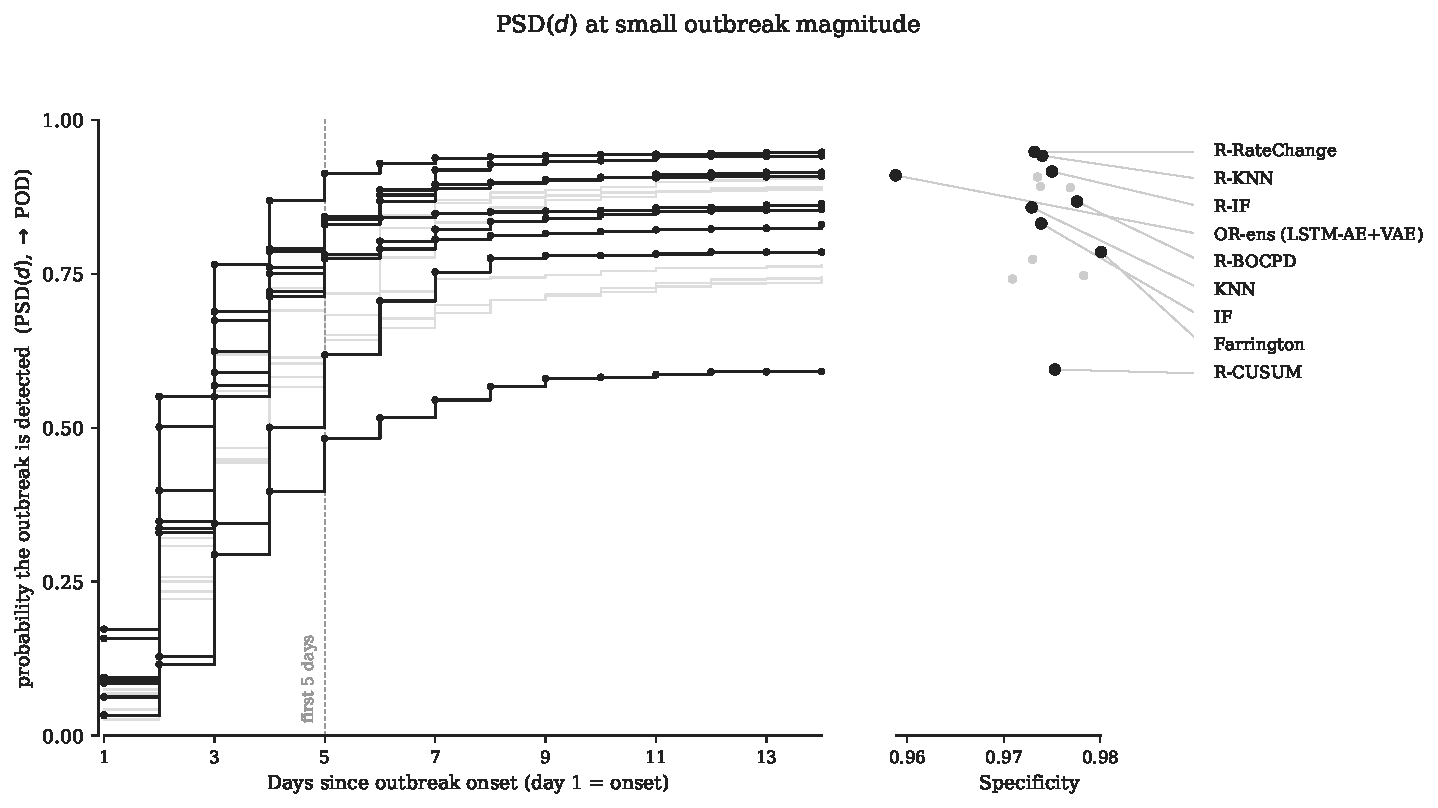
\includegraphics[width=\textwidth]{figs/tufte_timely_detection.pdf}}{%
  \fbox{\parbox{0.9\textwidth}{\centering\vspace{2em}Figure: PSD($d$) curves --- file \texttt{figs/tufte\_timely\_detection.pdf} not found.\vspace{2em}}}}
\caption{Timely detection at small outbreak magnitude, per simulation. \textbf{Left:} the Probability of Successful Detection within $d$ days, PSD($d$) --- each curve's asymptote is its POD and its early slope is its speed. \textbf{Right:} each method's specificity at the operating point, plotted at the same height (its POD) as its curve. PSD must be read against this panel: the OR-ensemble's high catch rate is bought at a lower specificity ($\approx$0.95) than the single detectors ($\approx$0.97--0.98), whereas RateChange matches its catch rate at essentially no specificity cost.}
\label{fig:psd}
\end{figure}

The picture differs markedly from the day-level sensitivity ranking (Table 1). Three findings stand out. First, the best OR-vote ensemble and the simple RateChange detector lead: each catches over 90\% of outbreaks within five days, with a conditional expected delay under two days. RateChange is striking --- it has the second-lowest day-level \textit{sensitivity} of any method (0.23, Table 1) yet near-best timely detection, because it is a pure onset detector: its fast-adapting EWMA baseline produces a large positive residual at the moment counts begin to climb, so it fires early, then falls silent as the baseline absorbs the elevated level. It flags few outbreak \textit{days} but catches the outbreak \textit{fast} --- exactly the property early warning rewards. The same mechanism explains why the change-point detector BOCPD, modest on day-level sensitivity (0.18), is the next-fastest method here (0.83 within five days).

Second, the methods reach their catch rate at very different speeds, and this reorders the single detectors relative to their day-level sensitivity. RateChange and the ensemble accrue most of their eventual detections within the first three days (0.77 and 0.74 within three days). The strongest single detectors by day-level sensitivity are slower to reach their asymptote: KNN and Isolation Forest reach only 0.57 and 0.55 within three days (conditional expected delay $\approx$ 2.2--2.3 days), and Farrington is slowest (CED 3.1 days; only 0.34 within three days, rising to 0.75 by day seven). Farrington eventually catches a fraction of outbreaks (POD 0.79) comparable to the faster detectors, but several days later. For a use case where intervention lead-time matters, this delay is consequential and is invisible to POD alone.

Third, CUSUM is the clear laggard on every horizon (0.48 within five days, CED 3.1 days). It is also the only method that detects \textit{worse} on longer outbreaks: its within-five-day PSD on outbreaks of 15+ days (0.49) is below its rate on 8--14-day outbreaks (0.68 catch rate), because its sequential statistic resets once the baseline adapts to a sustained elevation. CUSUM should not be relied upon as a standalone early-warning detector.

\tabcap{Table 11M.}{Timely detection at \textit{medium} outbreak magnitude, per simulation ($n = 1{,}598$ outbreaks). Methods sorted by PSD within five days.}

\begin{center}
\fitwidth{%
\begin{tabular}{lcccccc}
\toprule
Method & within 1 d & within 3 d & within 5 d & within 7 d & CED (days) & POD \\
\midrule
RateChange & 0.19 & 0.85 & \textbf{0.97} & 0.98 & \textbf{1.29} & 0.99 \\
OR-ensemble (IF + LSTM-AE + NB-HMM) & 0.14 & 0.82 & \textbf{0.97} & 0.99 & 1.53 & \textbf{0.99} \\
BOCPD & 0.18 & 0.79 & 0.92 & 0.94 & 1.48 & 0.95 \\
IF & 0.07 & 0.70 & 0.90 & 0.94 & 2.01 & 0.95 \\
KNN & 0.07 & 0.70 & 0.87 & 0.92 & 2.03 & 0.94 \\
VAE & 0.06 & 0.77 & 0.87 & 0.96 & 1.97 & 0.97 \\
NB-HMM & 0.06 & 0.60 & 0.86 & 0.91 & 2.10 & 0.92 \\
LOF & 0.02 & 0.63 & 0.84 & 0.89 & 2.25 & 0.91 \\
OCSVM & 0.07 & 0.60 & 0.82 & 0.88 & 2.50 & 0.91 \\
Farrington ($\alpha = 0.01$) & 0.03 & 0.51 & 0.78 & 0.91 & 2.74 & 0.93 \\
LSTM-AE & 0.04 & 0.60 & 0.77 & 0.83 & 2.38 & 0.87 \\
CUSUM & 0.00 & 0.19 & 0.51 & 0.59 & 3.66 & 0.65 \\
\bottomrule
\end{tabular}
}
\end{center}

\begin{figure}[ht]
\centering
\IfFileExists{figs/tufte_timely_detection_medium.pdf}{%
  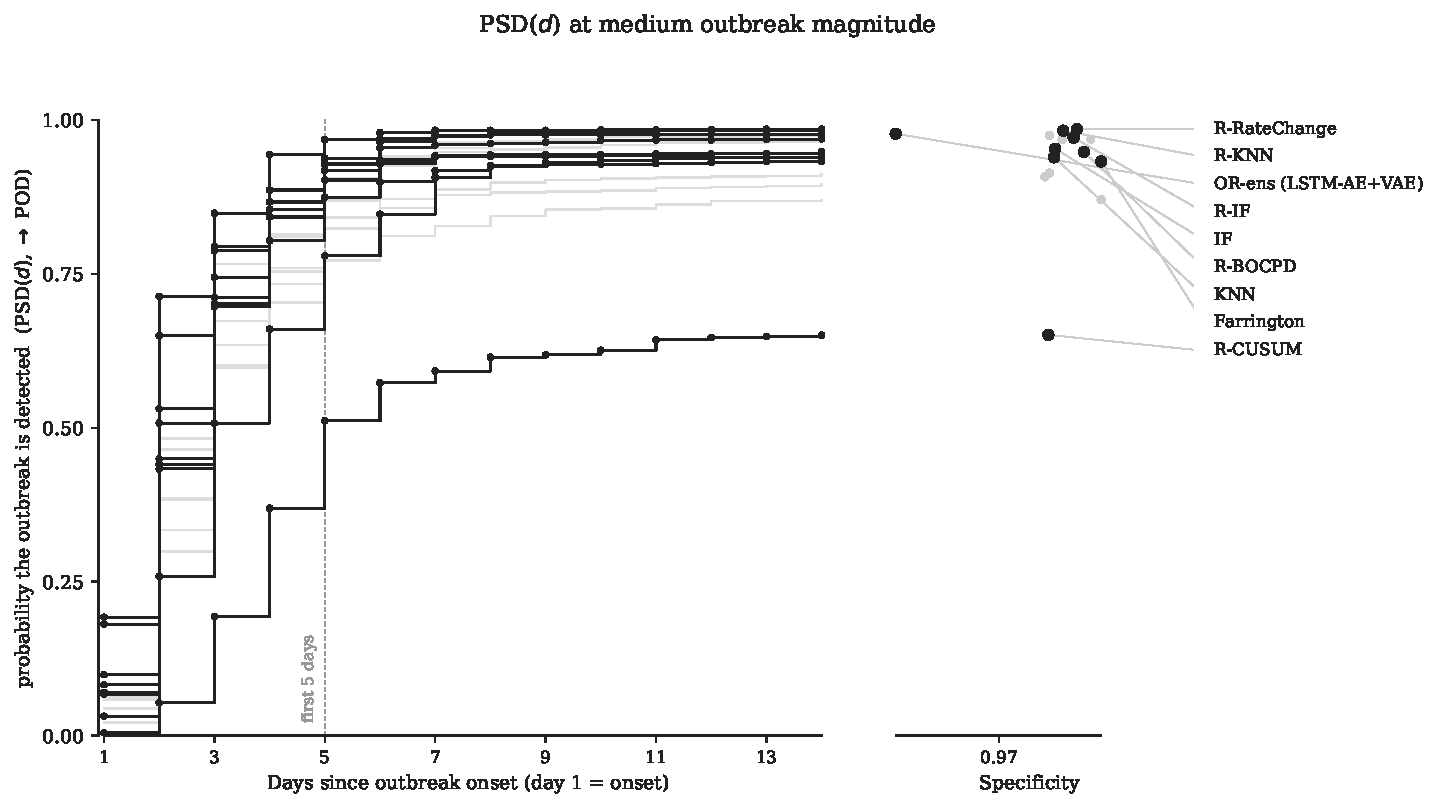
\includegraphics[width=\textwidth]{figs/tufte_timely_detection_medium.pdf}}{%
  \fbox{\parbox{0.9\textwidth}{\centering\vspace{2em}Figure: PSD($d$) curves at medium magnitude --- file \texttt{figs/tufte\_timely\_detection\_medium.pdf} not found.\vspace{2em}}}}
\caption{Timely detection at medium outbreak magnitude, per simulation. Layout as in Figure~\ref{fig:psd}.}
\label{fig:psd-medium}
\end{figure}

\tabcap{Table 11L.}{Timely detection at \textit{large} outbreak magnitude, per simulation ($n = 1{,}600$ outbreaks). Methods sorted by PSD within five days.}

\begin{center}
\fitwidth{%
\begin{tabular}{lcccccc}
\toprule
Method & within 1 d & within 3 d & within 5 d & within 7 d & CED (days) & POD \\
\midrule
OR-ensemble (IF + LSTM-AE + NB-HMM) & 0.18 & 0.89 & \textbf{0.99} & 0.995 & 1.18 & 0.995 \\
RateChange & 0.33 & 0.92 & 0.99 & 0.996 & \textbf{0.89} & \textbf{0.996} \\
IF & 0.09 & 0.85 & 0.985 & 0.99 & 1.47 & 0.99 \\
BOCPD & 0.30 & 0.89 & 0.98 & 0.99 & 1.00 & 0.99 \\
OCSVM & 0.07 & 0.80 & 0.98 & 0.99 & 1.61 & 0.99 \\
KNN & 0.06 & 0.81 & 0.97 & 0.98 & 1.51 & 0.98 \\
LOF & 0.03 & 0.77 & 0.95 & 0.96 & 1.74 & 0.97 \\
VAE & 0.11 & 0.84 & 0.94 & 0.99 & 1.57 & 0.99 \\
NB-HMM & 0.07 & 0.76 & 0.94 & 0.97 & 1.75 & 0.97 \\
Farrington ($\alpha = 0.01$) & 0.04 & 0.73 & 0.94 & 0.99 & 1.96 & 0.99 \\
LSTM-AE & 0.06 & 0.75 & 0.92 & 0.94 & 1.78 & 0.95 \\
CUSUM & 0.00 & 0.05 & 0.30 & 0.50 & 4.67 & 0.57 \\
\bottomrule
\end{tabular}
}
\end{center}

\begin{figure}[ht]
\centering
\IfFileExists{figs/tufte_timely_detection_large.pdf}{%
  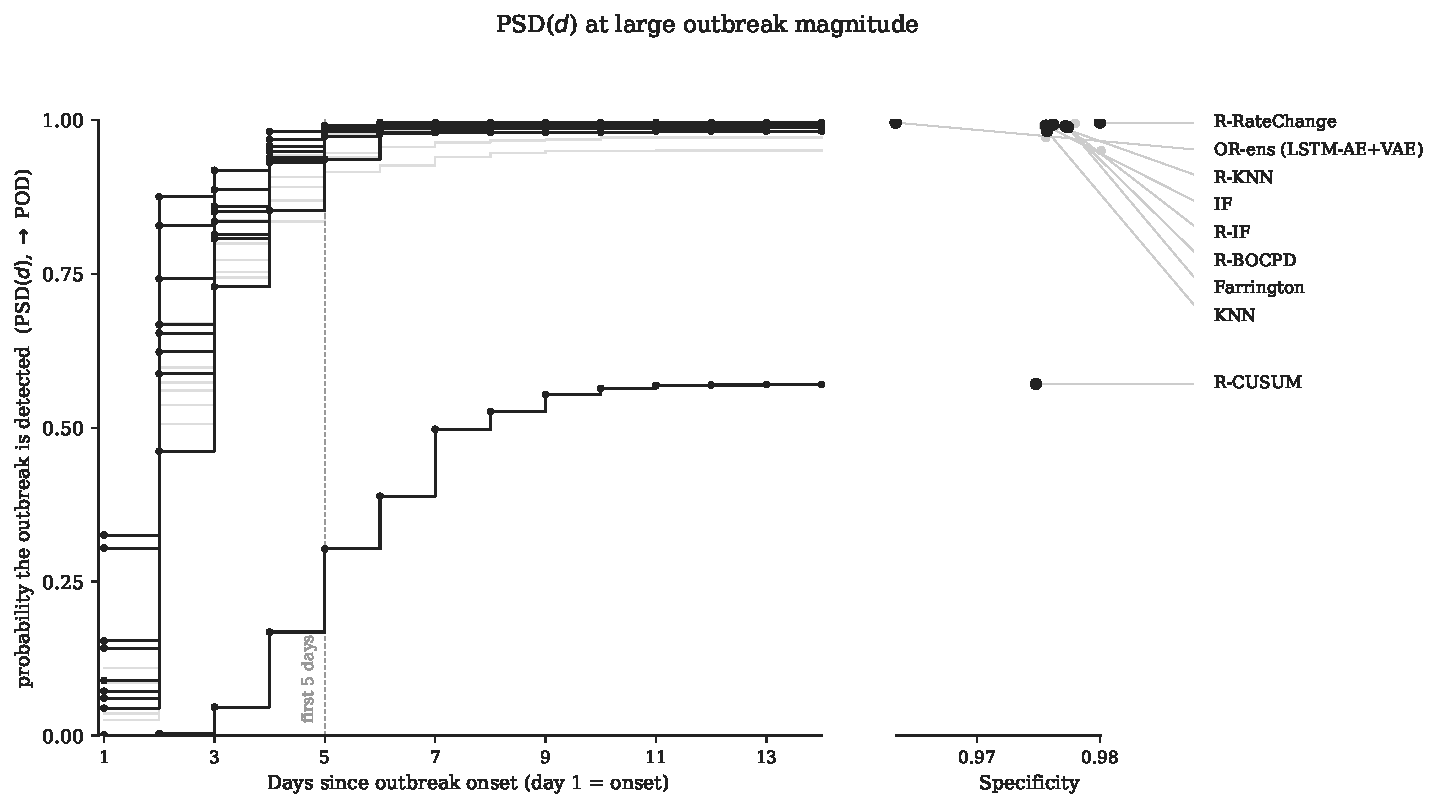
\includegraphics[width=\textwidth]{figs/tufte_timely_detection_large.pdf}}{%
  \fbox{\parbox{0.9\textwidth}{\centering\vspace{2em}Figure: PSD($d$) curves at large magnitude --- file \texttt{figs/tufte\_timely\_detection\_large.pdf} not found.\vspace{2em}}}}
\caption{Timely detection at large outbreak magnitude, per simulation. Layout as in Figure~\ref{fig:psd}.}
\label{fig:psd-large}
\end{figure}

The cross-magnitude PSD picture is consistent with, but more informative than, the day-level sensitivity story. At medium magnitude the small-magnitude ranking is preserved at the top --- RateChange and the OR-ensemble lead with PSD-within-5 of 0.97, BOCPD trails just behind (0.92), and the four tabular detectors cluster between 0.82 and 0.90 --- but the absolute catch rates of every method except CUSUM lift to between 0.78 and 0.97. At large magnitude eleven of the twelve detectors catch over 90\% of outbreaks within five days, the CEDs compress into a narrow band of 0.9--2.0 days, and the headline ordering is therefore dominated by sub-day differences (RateChange and BOCPD now post sub-second-day CEDs because their onset-sensitive mechanisms fire almost immediately on the strong large-magnitude shock). The exception across both magnitudes is CUSUM, which not only fails to scale (PSD-within-5 falls from 0.51 at medium to 0.30 at large, CED rises from 3.66 to 4.67 days) but uniquely degrades, confirming the small-magnitude finding that its sequential statistic is the wrong mechanism for sudden-onset events. For early-warning deployment the implication is that \textit{which} detector to pick matters most at small magnitude, where the gap between the fastest detector (RateChange, PSD-within-5 of 0.91) and the slowest non-CUSUM detector (Farrington, 0.62) spans 29 percentage points; at large magnitude almost any non-CUSUM choice catches the outbreak inside a week.

\subsection{Robustness: detectors without a fitted baseline}

The four residual-based detectors depend on the seasonal baseline of Section 3.3, whose harmonic functional form is of the same broad class as the data-generating process. To test whether their behaviour --- and the conclusions drawn from it --- relies on that fitted baseline, the three single-series statistical detectors (RateChange, CUSUM, BOCPD) were re-run with the parametric GLM replaced by a model-free, label-free deseasonaliser. For each day $t$ with weekday phase $w = t \bmod 7$, the count is standardised against the $K = 8$ most recent \textit{earlier} days of the same weekday,
\[
\tilde{r}_t = \frac{y_t - \operatorname{mean}(y_{\mathcal{H}_t})}{\max\!\big(\operatorname{std}(y_{\mathcal{H}_t}),\,1\big)},
\qquad \mathcal{H}_t = \{t-7,\, t-14,\, \dots\},
\]
which removes the weekly cycle and --- because the trailing window is short relative to the year --- the slow annual level, without fitting any model, estimating any seasonal parameters, or using any outbreak labels. NB-HMM has no model-free form (its emissions are defined relative to the fitted baseline mean) and is omitted; Farrington is the deployed reference and is unchanged. Everything else (the validation-based threshold tuning, the splits, and the evaluation) is identical to the fitted pipeline, so the two columns are directly comparable.

\tabcap{Table 13.}{Single-series statistical detectors under the fitted seasonal baseline versus the model-free deseasonaliser. Sensitivity is reported at all three magnitudes; specificity stays in the $0.97$--$0.98$ band throughout. Small-magnitude timeliness is shown for reference.}

\begin{center}
\fitwidth{%
\begin{tabular}{llcccc}
\toprule
Detector & Baseline & Sens (S) & Sens (M) & Sens (L) & Tim (S) \\
\midrule
RateChange & fitted GLM & 0.234 & 0.272 & 0.294 & 0.153 \\
RateChange & model-free & 0.188 & 0.218 & 0.249 & 0.251 \\
\addlinespace
CUSUM & fitted GLM & 0.404 & 0.460 & 0.393 & 0.533 \\
CUSUM & model-free & 0.243 & 0.307 & 0.315 & 0.723 \\
\addlinespace
BOCPD & fitted GLM & 0.175 & 0.212 & 0.291 & 0.198 \\
BOCPD & model-free & 0.133 & 0.154 & 0.202 & 0.290 \\
\bottomrule
\end{tabular}
}
\end{center}

Removing the fitted baseline lowers each detector but does not break it: all three remain functional and retain specificity in the $0.97$--$0.98$ band. The cost is uneven and informative. RateChange is barely affected on sensitivity ($-0.05$ at every magnitude) and stays the fastest single detector by conditional expected delay at all three magnitudes ($1.71$, $1.51$, $1.14$ days; the fitted version is $1.62$ at small), so its onset-detection \textit{speed} does not depend on a fitted model. Its catch rate does fall, however --- its probability of detection within five days at small magnitude drops from $0.91$ to $0.80$ --- and because the model-free deseasonaliser lowers RateChange's catch rate more than that of the tabular detectors (which never used the baseline), Isolation Forest overtakes it on the within-five-days metric at medium and large magnitude ($0.90$ and $0.985$ versus RateChange's $0.89$ and $0.965$). RateChange therefore remains the best single detector for timely detection at small magnitude and the fastest at every magnitude, but is no longer the leader on the combined within-five-days metric once outbreaks are large. CUSUM leans on the baseline most ($-0.16$ at small magnitude), though under the model-free stream it scales \textit{positively} with magnitude ($0.243 \to 0.315$) where the fitted version was flat-to-declining, indicating that the fitted baseline was propping up its small-magnitude numbers. BOCPD sits in between. The qualitative conclusions of Section 4.3 --- that these detectors are onset-sensitive, high-specificity, and complementary to the tabular methods --- are unchanged.

The same holds for the ensembles. Re-running the OR-vote search over the model-free statistical detectors plus the (unchanged) tabular, deep, and Farrington detectors still produces ensembles that clearly beat the best single detector (Table 14): the validation-selected ensemble reaches test sensitivity $0.715$ against $0.615$ for the best single detector (KNN), the same qualitative advantage reported in Section 4.5. The ceiling is lower than the fitted ensembles ($\approx 0.72$ versus $\approx 0.81$), and the gap is exactly the absent NB-HMM, the fitted-baseline detector that carried the headline fitted ensemble. Notably, the strongest GPU-free configuration, Farrington + IF + RateChange ($0.674$), is almost entirely model-free --- only the Farrington reference fits anything.

\tabcap{Table 14.}{Validation-selected OR-vote ensembles at small magnitude when the statistical detectors use the model-free deseasonaliser (NB-HMM excluded). Test metrics reported.}

\begin{center}
\fitwidth{%
\begin{tabular}{llccl}
\toprule
Selection constraint & Ensemble (val-selected) & Sensitivity & Specificity & Cost \\
\midrule
Max sensitivity (spec $\geq 0.93$) & Farrington + LSTM-AE + VAE & 0.715 & 0.940 & expensive \\
Highest-sens GPU-free (spec $\geq 0.93$) & Farrington + IF + RateChange & 0.674 & 0.939 & medium \\
Balanced (spec $\geq 0.95$) & LSTM-AE + VAE & 0.666 & 0.951 & expensive \\
Best all-cheap (spec $\geq 0.95$) & Farrington + IF & 0.627 & 0.960 & medium \\
\bottomrule
\end{tabular}
}
\end{center}

\begin{figure}[ht]
\centering
\IfFileExists{figs/tufte_nofit_timely.pdf}{%
  \includegraphics[width=\textwidth]{figs/tufte_nofit_timely.pdf}}{%
  \fbox{\parbox{0.9\textwidth}{\centering\vspace{2em}Figure: model-free PSD --- file \texttt{figs/tufte\_nofit\_timely.pdf} not found.\vspace{2em}}}}
\caption{Timely detection under the model-free pipeline at small magnitude: the statistical detectors run on the weekday rolling-z deseasonaliser, while the tabular, deep, and Farrington detectors are unchanged and NB-HMM is dropped. Layout as in Figure~\ref{fig:psd} --- left: PSD$(d)$, the probability of catching the outbreak within $d$ days, rising to each method's POD; right: the specificity that catch rate costs. At this (small) magnitude the model-free ensemble (Farrington + IF + RateChange) and RateChange lead on timely detection while CUSUM lags, as under the fitted pipeline (Figure~\ref{fig:psd}); at medium and large magnitude the tabular detectors overtake RateChange on this metric (Figures~\ref{fig:psd-nofit-medium} and~\ref{fig:psd-nofit-large}).}
\label{fig:psd-nofit}
\end{figure}

\begin{figure}[ht]
\centering
\IfFileExists{figs/tufte_nofit_timely_medium.pdf}{%
  \includegraphics[width=\textwidth]{figs/tufte_nofit_timely_medium.pdf}}{%
  \fbox{\parbox{0.9\textwidth}{\centering\vspace{2em}Figure: model-free PSD (medium) --- file not found.\vspace{2em}}}}
\caption{Timely detection under the model-free pipeline at \textit{medium} outbreak magnitude. Layout as in Figure~\ref{fig:psd-nofit}.}
\label{fig:psd-nofit-medium}
\end{figure}

\begin{figure}[ht]
\centering
\IfFileExists{figs/tufte_nofit_timely_large.pdf}{%
  \includegraphics[width=\textwidth]{figs/tufte_nofit_timely_large.pdf}}{%
  \fbox{\parbox{0.9\textwidth}{\centering\vspace{2em}Figure: model-free PSD (large) --- file not found.\vspace{2em}}}}
\caption{Timely detection under the model-free pipeline at \textit{large} outbreak magnitude. Layout as in Figure~\ref{fig:psd-nofit}. As under the fitted pipeline, CUSUM uniquely degrades on the strongest outbreaks (PSD-within-5 of $0.25$, conditional expected delay $4.1$ days) while the onset-sensitive detectors and the ensemble exceed $0.95$.}
\label{fig:psd-nofit-large}
\end{figure}

Taken together, the model-free results show that the headline findings of this study --- tabular methods lead among individual detectors, ensembles beat any single method at small magnitude, and the onset-sensitive detectors give the best timely detection --- do not depend on the fitted seasonal baseline. What the fitted baseline buys is \textit{absolute} sensitivity for the residual detectors (most for CUSUM, least for RateChange), not the qualitative ordering. The fitted pipeline is retained as the main analysis because it runs each method at its standard, intended operating point; this model-free variant brackets the opposite extreme and confirms the relative conclusions transfer across the choice of baseline.


\section{Discussion}

\subsection{Feature engineering is more important than model complexity}

The most striking result is that density and distance-based methods operating on hand-crafted tabular features outperform more complex deep learning architectures. At large outbreak magnitude, all four tabular methods exceed the VAE (0.611) and three of the four exceed LSTM-AE (0.816). The 20-dimensional feature vector, which encodes rolling summary statistics and lag differences, captures the local statistical context that distinguishes outbreak days from the seasonal baseline. This finding is consistent with the broader machine learning literature, in which feature engineering often dominates model selection for tabular data.

The tabular methods also exhibit the strongest scaling with outbreak magnitude. Isolation Forest gains +0.304 sensitivity from small to large, the largest absolute improvement of any method. This suggests that the point-anomaly inductive bias --- ``this day's feature vector is unusual relative to the training distribution'' --- is well-matched to outbreak detection on count data, where outbreak peaks create feature vectors that are increasingly separable from the baseline as the outbreak signal strengthens.

The residual-feature ablation (Section 4.6) reinforces this conclusion from a different direction. Changing only the input representation --- replacing raw counts with Pearson residuals from a seasonal baseline, while holding the detector, features, and tuning fixed --- improves sensitivity on strongly seasonal signals for every one of the four tabular detectors (by +0.075 to +0.225). The detectors were never the bottleneck on these signals; the raw-count features were, because they confounded the seasonal cycle with outbreaks. This is direct evidence that the representation, not the model, governs performance in this setting.

\subsection{The value of OR-vote ensembles is greatest at small magnitudes}

At small outbreak magnitude, optimising any single detector yields at most sensitivity 0.615 (KNN). The OR-vote ensemble of four detectors from different families (Farrington + IF + LSTM-AE + NB-HMM) reaches 0.783, a gain of 17 percentage points that a paired cluster bootstrap confirms is statistically reliable (Section 4.5). At large magnitude, however, the gap narrows sharply: KNN alone achieves 0.854, while the best ensemble reaches 0.902 (Table 3) --- a margin of only about five points. This pattern arises because at low signal-to-noise, different detection families succeed on different subsets of simulations and signals, and OR-voting captures the union of these successes; at high signal-to-noise, the outbreak signal is strong enough that most methods detect it, and the marginal value of additional detectors diminishes. The ensemble is therefore most valuable precisely in the operationally hardest regime --- small, subtle outbreaks.

This finding has practical implications. For surveillance systems that must detect outbreaks across a range of magnitudes, including small ones, ensemble strategies provide a substantial and otherwise unattainable performance gain. For systems operating in settings where outbreaks are expected to be large (e.g., monitoring for pandemic-scale events), a well-tuned individual detector such as KNN or Isolation Forest may suffice.

\subsection{Statistical baseline methods occupy a distinct niche}

The five methods that share the Negative Binomial seasonal baseline (CUSUM, BOCPD-residual, NB-HMM, RateChange, Farrington) span a wide performance range (sensitivity 0.175 to 0.522 at small magnitude). NB-HMM is the strongest, consistently outperforming Farrington by 8--10 sensitivity points at every magnitude. The hidden-state formulation of NB-HMM appears to extract more information from the baseline residuals than the single-day testing approach (Farrington) or the cumulative accumulation approach (CUSUM).

CUSUM exhibits flat sensitivity across magnitudes (0.404, 0.460, 0.393), an unexpected result given that larger outbreaks produce larger residuals. The explanation is that both the slack parameter $k$ and the alarm threshold are re-tuned per magnitude, so that gains from larger signals are offset by tighter thresholds. Timeliness remains poor for CUSUM (approximately 0.5), as the cumulative-sum mechanism requires several days of elevated counts before triggering. BOCPD-residual slightly degrades with increasing magnitude ($-0.033$), likely because the Gaussian approximation to the Pearson residuals becomes less accurate when extreme counts from large outbreaks inflate the residuals.

Despite their lower individual sensitivity, statistical baseline methods contribute meaningfully to ensemble performance. Farrington and NB-HMM, which operate on a fundamentally different signal (NB quantile exceedance and HMM state posterior, respectively) than the tabular feature-space methods, provide complementary detection coverage that improves OR-vote ensembles beyond what is achievable with tabular methods alone.

\subsection{Reconstruction-based deep learning methods are competitive but not dominant}

LSTM-AE achieves the most consistent ranking of any individual detector, appearing in the top five at every magnitude. However, its sensitivity is surpassed by KNN and Isolation Forest at large outbreaks (0.816 vs.\ 0.854 and 0.827, respectively). The VAE with Negative Binomial output achieves the best timeliness of any reconstruction-based method (0.080 at large magnitude) but lags behind the tabular methods in sensitivity at every magnitude (0.424, 0.516, 0.611). The reconstruction-based approach --- detecting anomalies as days that are poorly reconstructed by a model trained on normal data --- is sound in principle but appears less effective than the direct density estimation performed by the tabular methods on this dataset.

Both deep learning methods require GPU hardware for training, placing them in the \textit{expensive} cost tier. Given that the tabular methods achieve comparable or superior performance without GPU requirements, the practical case for deep learning detectors in this setting rests on their contribution to ensemble diversity rather than their individual performance.

\subsection{Per-signal variation reveals complementary strengths across method families}

The per-signal analysis (Section 4.3) provides an important qualification to the aggregate results: no single method is uniformly best across all 16 signals. The best-performing method varies by signal, with tabular methods excelling on signals with strong seasonal structure (herpes zoster, upper respiratory tract infection) and statistical methods excelling on signals with well-characterised Negative Binomial dynamics (hepatitis, ICU cardiac admissions). This complementarity provides the mechanistic explanation for why OR-vote ensembles outperform any individual method --- the ensemble captures the union of per-signal strengths.

The existence of consistently hard signals (heat stroke, insect bites, ILI --- all with mean sensitivity below 0.35 at small magnitude) suggests that these signals may require signal-specific modelling approaches or alternative feature representations. The convergence of per-signal sensitivity at large magnitude --- the coefficient of variation for KNN drops from 0.36 to 0.06 --- provides reassurance that the hard signals are not fundamentally undetectable, but rather that their outbreak signatures are subtle at low magnitude.

A correlation analysis between per-signal detection performance and signal characteristics computed from the training data identifies three properties that govern which family succeeds on which signal. First, \textit{seasonal amplitude} is the dominant predictor for the tabular and deep-learning methods: the rank correlation between a signal's relative seasonal amplitude and detector sensitivity is strongly negative for Isolation Forest ($\rho = -0.53$), KNN ($\rho = -0.54$), and OCSVM ($\rho = -0.57$), confirming the mechanism behind the residual-feature improvement. Second, \textit{outbreak signal-to-noise ratio} is the dominant predictor for the statistical methods, which detect departures from a fitted baseline and therefore require the outbreak to exceed the residual noise floor: the correlation is strongly positive for NB-HMM ($\rho = +0.67$) and BOCPD-residual ($\rho = +0.80$). Third, \textit{overdispersion} (the variance-to-mean ratio of the baseline counts) is strongly negative for the residual-based statistical detectors --- CUSUM ($\rho = -0.56$) and NB-HMM ($\rho = -0.50$) --- because high baseline variability inflates the null distribution and raises the effective detection threshold. These three properties explain the complementarity exploited by the ensemble: the tabular and statistical families fail on disjoint sets of signals (those with strong seasonality versus those with low outbreak signal-to-noise), so their union covers more signals than either alone.

CUSUM's extreme signal-dependence (sensitivity ranging from 0.000 on bronchitis to 0.697 on pertussis) warrants particular attention. The cumulative-sum mechanism is effective for signals where outbreaks manifest as gradual, sustained elevations, but fails catastrophically on signals with different outbreak profiles. This makes CUSUM unsuitable as a standalone detector in a multi-signal surveillance system.

\subsection{Comparison with supervised methods}

A natural question is how these unsupervised methods compare to a supervised detector that has access to outbreak labels at training time. A companion analysis (reported separately) trains a supervised stacked meta-learner on the outputs of the individual detectors; its principal advantage over the unsupervised ensembles is specificity, since by learning the explicit boundary between outbreak and non-outbreak days it can suppress false alarms more aggressively than an unsupervised OR-vote. On sensitivity, however, the best unsupervised ensemble (Farrington + IF + LSTM-AE + NB-HMM, 0.783 at small magnitude) is competitive, and at large magnitude individual unsupervised detectors (KNN 0.854, IF 0.827) are strong in absolute terms. The practical argument for the unsupervised approach is that it requires no labelled outbreak examples at training time --- the decisive consideration for novel or emerging diseases, where such labels do not exist. A full quantitative supervised-versus-unsupervised comparison is left to the companion work, as the supervised stacker falls outside the unsupervised scope of this chapter.

For novel-outbreak detection on previously unseen signals --- the core use case for syndromic surveillance of emerging diseases --- the unsupervised approach is the more principled choice, as it does not require labelled outbreak examples for training.

\subsection{Limits of detectability and statistical uncertainty}

Three caveats bound the interpretation of the reported sensitivities. First, a substantial fraction of the injected outbreaks are not detectable by \textit{any} method, and this reflects the realism of the simulator rather than a deficiency of the detectors. Outbreaks are injected throughout the final year, including on weekends and public holidays when reporting volume is naturally low, and during seasonal troughs. After accounting for the day-of-week and seasonal structure of the baseline --- the same structure the seasonal-baseline methods model explicitly --- roughly one quarter to one third of injected outbreaks at small magnitude have peak counts that do not exceed the baseline expectation for that day. These outbreaks carry essentially no detectable signal, and they place a ceiling on achievable sensitivity that is well below 1.0. The reported aggregate sensitivities should therefore be read as performance over a mixture of detectable and (realistically) undetectable events, not as performance over a set of clearly anomalous days. This is a property of genuine syndromic data, in which reporting artefacts and low-season variability routinely obscure small aberrations.

A methodological point bears on how detectability should be characterised, and corrects an analysis reported in an earlier draft. Each simulation contains exactly one injected outbreak, whose true median duration is 16 days (96\% last eight days or more; Table 12). It is tempting to define an ``event'' as a maximal run of consecutive injected days and to study detection as a function of run length. Doing so is misleading here: because the per-day injected count follows a Negative-Binomial draw around a log-normal temporal profile, a single $\approx$2-week outbreak frequently has interior days with zero injected cases, so the run-based definition fragments one outbreak into a multi-day body plus several isolated single-day ``satellite'' runs. Under that definition 40\% of ``events'' appear to be single-day, and detection appears to rise steeply with run length --- but this is an artefact of fragmentation, not a property of the injected outbreaks. Merging runs separated by short zero-count gaps collapses the 4,831 apparent events to roughly 1,600 --- one per simulation, as injected --- and shifts the median apparent duration from two days to sixteen. The correct, per-simulation analysis therefore studies detection of the single outbreak, as the POD and timeliness metrics of \citet{noufaily2019} already do, and is the basis for the timely-detection results in Section 4.7.

\tabcap{Table 12.}{True distribution of injected-outbreak duration at small magnitude, computed per simulation (one outbreak each). Duration is the span from the first to the last injected day within the evaluation window.}

\begin{center}
\fitwidth{%
\begin{tabular}{lccccc}
\toprule
Outbreak duration & 1 day & 2--3 days & 4--7 days & 8--14 days & 15+ days \\
\midrule
Share of outbreaks & 0.8\% & 0.8\% & 2.1\% & 42.0\% & 54.4\% \\
\bottomrule
\end{tabular}
}
\end{center}

Because outbreak duration is therefore near-uniformly long (median 16 days), it is not a discriminating axis of difficulty in this dataset; what distinguishes the detectors is not \textit{which} outbreaks they catch by duration but \textit{how quickly} they catch them, which is precisely what the timely-detection metric of Section 4.7 measures. The genuine duration-related finding that survives the correction is narrow and method-specific: among the long outbreaks, most detectors do slightly better on 15+-day than on 8--14-day events, whereas CUSUM does \textit{worse} on the longest outbreaks, because its sequential statistic resets once the seasonal baseline adapts to a sustained elevation.

Second, with 100 test simulations per signal, per-signal sensitivity estimates carry meaningful sampling uncertainty. Bootstrap resampling yields 95\% confidence intervals on per-signal sensitivity with half-widths of approximately 3--5 percentage points for most methods. Consequently, per-signal differences smaller than this between two methods (for example, a 0.02--0.03 gap in a single cell of Table 6) should not be interpreted as meaningful. The aggregate, cross-signal comparisons are more precise; the qualitative conclusions --- the ordering of method families, the ensemble advantage at small magnitude, and the seasonal-signal benefit of residualisation --- are robust to this uncertainty, resting on differences that exceed the bootstrap confidence intervals (Section 4.5).

Third, and most importantly for external validity, all results derive from a single simulation framework. Although that framework \citep{noufaily2013} is the established standard for evaluating aberration-detection algorithms and its parameters were chosen to span the diversity of real surveillance streams, it remains a synthetic data-generating process. The \textit{absolute} sensitivities reported here should not be expected to transfer directly to real surveillance data, where outbreak shapes, reporting behaviour, and baseline dynamics are more heterogeneous and where the clean separation between training-period and outbreak-period data does not hold. The transportable contributions of this study are the \textit{relative} findings: the ordering of method families, the complementarity that underpins the ensemble advantage, the dependence of detection performance on signal seasonality and outbreak magnitude, the divergence between day-level sensitivity and timely detection (Section 4.7), and the demonstration that input representation rather than model complexity is the binding constraint. Validation on real surveillance data with confirmed outbreaks is the natural next step and is left to future work.

\subsection{Is timely detection the right metric?}

The timely-detection results (Section 4.7) reorder the methods enough to raise the question of which metric should anchor the evaluation. We argue that PSD($d$) is the most \textit{decision-relevant} detection metric for the early-warning use case, for three reasons, but that it is not a sufficient summary on its own.

First, it maps directly onto operational utility. A surveillance system exists to trigger an investigation before an outbreak grows; what matters is the probability of raising the alarm within a usable lead-time, which is exactly PSD($d$) at the operationally chosen horizon $d$. Day-level sensitivity, by contrast, rewards a detector for flagging \textit{every} day of an outbreak --- but once the first alarm has fired and an investigation is underway, the subsequent daily alarms carry little additional operational value. This is why RateChange, which flags few outbreak days (sensitivity 0.23) but catches the onset quickly (91\% within five days), is far more useful for early warning than its day-level sensitivity suggests, and why day-level sensitivity can actively mislead method selection for this purpose.

Second, PSD decomposes cleanly into the two things a decision-maker cares about. Its asymptote is the catch rate (POD: will we detect this at all?) and its early slope is the speed (how soon?). The existing timeliness metric (Section 2.3) entangles these --- it mixes the lateness of caught outbreaks with a unit miss-penalty, and normalises by outbreak length, so a change in the score cannot be attributed to either cause and is not comparable across signals with different outbreak durations. PSD reports the delay on an absolute, interpretable day scale and separates ``missed'' from ``late''.

Third, it is grounded in the established theory of statistical surveillance \citep{frisen2003, sonesson2003}, where the probability of timely detection and the conditional expected delay are the standard optimality criteria for sequential change detection, alongside the in-control run length (the false-alarm analogue). This places the metric on the same footing as the literature our Farrington and CUSUM baselines come from.

That said, PSD is not a complete one-number summary, for the same reason no detection metric is: it says nothing about false alarms. PSD can be driven to 1 by a detector that alarms constantly, so it is interpretable only at a controlled specificity --- which is why we tune every method to a common specificity floor and report PSD at that operating point. The honest single summary of a detector for early warning is therefore a \textit{pair}: timely-detection skill (PSD at an operational $d$, or equivalently the CED) together with the false-alarm rate it costs --- one chosen operating point on what is, in effect, a timeliness-versus-specificity trade-off. PSD also requires committing to a horizon $d$ (or reporting the whole curve and the CED), and its values depend on how outbreak onset is defined. Within those bounds, it is the metric that best captures the purpose of the system, and we recommend it --- paired with specificity --- as the primary basis for comparing detectors intended for early warning, with day-level sensitivity retained as a secondary, complementary characterisation of how completely the outbreak signal is tracked once detected.


\section{Conclusion and Recommendations}

This study compared 11 unsupervised anomaly detection methods and their OR-vote ensembles on simulated syndromic surveillance data across three outbreak magnitudes. The principal findings are:

\begin{enumerate}
\item Density and distance-based methods on a 20-dimensional tabular feature space (KNN, Isolation Forest, LOF, OCSVM) constitute the strongest individual detectors, with KNN achieving the highest sensitivity at large outbreaks (0.854) and all tabular methods exhibiting the strongest positive scaling with outbreak magnitude.

\item OR-vote ensembles combining detectors from different methodological families substantially outperform any individual method at small outbreak magnitudes, reaching test sensitivity 0.77--0.78 (at specificity $\approx 0.93$) against 0.615 for the best single detector. The advantage is statistically reliable (paired cluster bootstrap over 16 signals, 95\% CI on the ensemble--KNN difference $[+0.038, +0.186]$) but is purchased at a specificity cost (ensembles operate near 0.93--0.95 versus $\approx 0.97$ for single detectors), and it diminishes at large magnitudes, where individual tabular methods approach ensemble performance.

\item Ensemble configurations were selected on the validation partition and reported on the test partition to avoid selection-on-test bias; this and the correction of an alarm-magnitude alignment error reduced the Farrington-containing ensemble figures by 8--17 percentage points relative to an earlier test-selected analysis. After correction, the strongest high-sensitivity ensemble is Farrington + IF + LSTM-AE + NB-HMM (test sensitivity 0.783), with the Farrington-free IF + LSTM-AE + NB-HMM close behind (0.770); the most economical competitive option is Farrington + IF + NB-HMM (0.725, no GPU). The all-cheap statistical ensemble Farrington + NB-HMM attains the highest specificity (0.962) at sensitivity 0.615.

\item CUSUM and BOCPD-residual do not benefit from larger outbreaks and should not be relied upon as standalone detectors. NB-HMM is the strongest statistical detector, consistently outperforming Farrington by 8--10 sensitivity points.

\item Deep learning methods (LSTM-AE, VAE) are competitive individual detectors but do not justify their computational cost for this dataset. Their primary value is as ensemble diversity contributors.

\item Detection performance varies substantially across signals, with consistently hard signals (heat stroke, insect bites, ILI) achieving mean sensitivity below 0.35 at small magnitude across all methods. No single method is best on all signals; the tabular and statistical method families have complementary per-signal strengths, providing the mechanistic basis for the ensemble advantage. At large magnitude, per-signal variation is substantially reduced for the tabular and deep learning methods, but CUSUM and NB-HMM retain high signal-dependence. A correlation analysis identifies three signal properties that govern method success: seasonal amplitude (negatively predicts tabular-method performance), outbreak signal-to-noise ratio (positively predicts statistical-method performance), and overdispersion (negatively predicts residual-based statistical methods).

\item Replacing raw counts with seasonal-baseline residuals as the input to the tabular detectors improves sensitivity by approximately +0.15 on strongly seasonal signals (Isolation Forest and KNN) with negligible effect on low-seasonal signals. A conditional policy that residualises only seasonal signals raises mean Isolation Forest sensitivity from 0.523 to 0.593 at small magnitude with no per-signal regressions, demonstrating that input representation, rather than model complexity, is the binding constraint on these signals.

\item For early warning, \textit{timely} detection rather than day-level sensitivity is the decision-relevant criterion, and it reorders the methods. Measured per simulation (each carries one injected outbreak, median duration 16 days), the probability of detecting the outbreak within five days of onset is highest for the IF + LSTM-AE + NB-HMM ensemble (0.93) and the simple onset-sensitive RateChange detector (0.91, conditional expected delay 1.6 days) --- the latter despite having the second-lowest day-level sensitivity, because it fires fast at outbreak onset then falls silent. Farrington is comparatively slow (expected delay 3.1 days) and CUSUM is the weakest on every horizon and uniquely degrades on the longest outbreaks. We recommend the probability of successful detection within $d$ days (PSD; \citealp{frisen2003}), reported alongside specificity, as the primary metric for comparing early-warning detectors, with day-level sensitivity retained as a complementary measure. An earlier draft's claim that ``outbreak duration is the primary determinant of detectability'' was an artefact of fragmenting each single $\approx$2-week outbreak into spurious single-day events and does not survive a per-simulation analysis (Section 5.7).
\end{enumerate}

Table 9 summarises the recommended configurations for different deployment scenarios.

\tabcap{Table 9.}{Recommended configurations for different deployment scenarios. Sensitivity and timeliness are reported as (small / medium / large) magnitude.}

\begin{center}
\fitwidth{%
\begin{tabular}{llcccl}
\toprule
Scenario & Recommended method & Sensitivity & Timeliness & FPR & Cost \\
\midrule
Maximum sensitivity (any cost) & Farrington + IF + LSTM-AE + NB-HMM (OR-vote) & 0.783 / 0.857 / 0.903 & 0.141 / 0.094 / 0.059 & 0.068 & expensive \\
Best overall, GPU-free & Farrington + IF + NB-HMM (OR-vote) & 0.725 / --- / --- & 0.095 / --- / --- & 0.055 & medium \\
Highest specificity ensemble & Farrington + NB-HMM (OR-vote) & 0.615 / --- / --- & 0.226 / --- / --- & 0.038 & cheap \\
Best single detector & KNN (per-signal tuned) & 0.615 / 0.750 / 0.854 & 0.281 / 0.178 / 0.099 & 0.027 & medium \\
Best single detector, seasonal-heavy signals & KNN on seasonal-baseline residuals & 0.701 / 0.805 / 0.857 & --- & ${\sim}0.027$ & medium \\
Lightweight single model & Isolation Forest (per-signal tuned) & 0.523 / 0.678 / 0.827 & 0.291 / 0.162 / 0.085 & 0.026 & medium \\
Lightweight, seasonal-heavy signals & Isolation Forest, conditional residual features & 0.593 / 0.743 / 0.845 & --- & ${\sim}0.026$ & medium \\
Interpretable statistical baseline & NB-HMM & 0.522 / 0.633 / 0.731 & 0.310 / 0.181 / 0.106 & 0.027 & cheap \\
Traditional reference & Farrington ($\alpha = 0.01$) & 0.440 / 0.556 / 0.639 & 0.378 / 0.215 / 0.128 & 0.020 & cheap \\
\bottomrule
\end{tabular}
}
\end{center}

These results support the adoption of heterogeneous unsupervised ensembles for syndromic surveillance of emerging diseases, where labelled outbreak data are unavailable at training time and detection must be robust across unknown outbreak magnitudes. These conclusions are established on a single, widely-used simulation framework; their relative orderings and mechanisms are expected to transfer, but validation on real surveillance data with confirmed outbreaks remains an essential next step before operational deployment.


\nocite{buckinghamjeffery2017}
\bibliographystyle{plainnat}
\bibliography{references}

\end{document}
